\documentclass[a4paper]{book}
%\documentclass[a4paper,draft]{book}

%%%% Basics %%%%
\usepackage[ngerman]{babel}
\usepackage[utf8]{inputenc}
\usepackage[T1]{fontenc}
% \usepackage[top=2.5cm,bottom=1.75cm,right=2cm,left=2.3cm]{geometry}
% \usepackage{wrapfig}


%%%% Bilder %%%%
\usepackage{graphicx}
%% \usepackage{floatflt} 
\usepackage{subfigure} 


%%%% Mathe %%%%
\usepackage{amsmath}
\usepackage{amssymb}
\usepackage{units}


%%% Programmieren %%%
\usepackage{listings} 
\lstset{numbers=left,numberstyle=\tiny,numbersep=5pt,breaklines=true,basicstyle=\small}  
\lstset{language=c++} 
%% Als Code-Schnippsel im Fließtext
% \lstinline|print "hello world"|
%% Als eigenständigen Sourcecode
% \begin{lstlisting}[caption=Beispielcode]{Name}
% print "hello world";
% \end{lstlisting}
%% Einbetten einer externen Source-Code-Datei
% \lstinputlisting[frame=single,label=beispielcode,caption=Ein Beispiel]{beispiel.pl} 


%%%% Spalten %%%%
\usepackage{multicol}
% zu verwenden mit \begin{multicols}{3} 3 steht fuer die
%    spalenzahl \end{multicols}


%%%% Zeilenabstand %%%%
% \setlength{\parindent}{0pt} %Absatz-Einrückung
% \setlength{\parskip}{12pt} %Absatz-Abstände
%% oder
% \usepackage{setspace} %Zeilenabstand bestimmbar in Dokumentenabschnitten
%% oder
% \linespread{$$Verhältnis_zu_normalem_Zeilenabstand$$} %Wirkt global
\newcommand{\abs}{\bigskip \noindent}


%%%% Tabellen %%%%
\usepackage{booktabs}
\setlength{\tabcolsep}{5pt} 
    %Abst zw Spalten
\renewcommand{\arraystretch}{1.4}
    %Vielfacher Spaltenabst zw Zeilen


%%%% Aufzaehlungen %%%%
%% description
\usepackage{expdlist}
    %mehr Moeglichkeiten
%% enumerate
\usepackage{enumerate}
    %individuelle Aufzaehlungen
    %nach \begin{enumerate}[(a)] erzeugt (a).. (b).., ...
    %entsprechend mit (i) (A) (I) 1. Nr 1 usw.


%%%% Kopfzeile %%%%
\usepackage{fancyhdr} 
% \pagestyle{myheadings} %Kopfzeile hinzufügen
%\markright{$$Kopfzeile$$} %Inhalt der Kopfzeile
%%
%\pagestyle{fancy} %Genauer zu definierende Kopfzeile
%\fancyhead[OL,OC,OR,EL,EC,ER]{} %O: ungerade seiten, E: gerade Seiten,
%\fancyfoot[OL,OC,OR,EL,EC,ER]{} %L:Links, C:Mitte, R:Rechts (leere Klammer {} löscht)
%\renewcommand{\headrulewidth}{dicke} %Dicke der Linie oben
%\renewcommand{\footrulewidth}{dicke} %Dicke der Linie unten
%\addtolength{\headwidth}{länge} %Breite wird vergrößert (ragt über Text raus)
%\addtolength{\headheight}{länge} %Höhe wird vergrößert


%%%%% Ueberschriften %%%%
%\setcounter{secnumdepth}{4} 
    %Paragraph wird nummeriert
%\def\theparagraph{\textit{\mdseries\underline{\roman{paragraph}.}}}
%\def\theparagraph{$\rhd$ (\alph{paragraph})} 
    %Paragraph bekommt statt nummer ein Dreieck

%% bei scrbook %%
% \usepackage{sectsty}
% \paragraphfont{\sffamily}


%%%% Andere Nummerierungen %%%%
%\def\thefigure{\arabic{section}.\arabic{figure}\textsuperscript{\arabic{page}}}
%\def\theequation{\arabic{section}.\arabic{equation}\textsuperscript{\arabic{
%page}}}


%%%% Referenzen %%%%
%\usepackage[german]{varioref}
% mit \vref{label} wird eine individuelle 
% Bezeichnung verwendet; je nach dem,
% wie weit label und vref auseinander liegen.


%%%% Links %%%%
\usepackage[colorlinks=true,linkcolor=black,citecolor=black,%
bookmarksnumbered=true,breaklinks=true,pdfstartview=FitH]{hyperref}


%%%% Index %%%%
%\usepackage{makeidx}
%\makeindex



%%%% Eigene Komandos %%%%
\newcommand{\zitat}[1]{{\slshape \sffamily #1}} 
%hebt Zitate deutlich ab
\newcommand{\diff}{\ensuremath{\operatorname d}}
\newcommand{\Ve}[1]{\ensuremath{\vec{#1}}}
\renewcommand{\vec}[1]{\ensuremath{\boldsymbol{#1}}}
\newcommand{\Grad}{\ensuremath{\operatorname{grad}}}
\newcommand{\Mat}[1]{\ensuremath{\mathbf{#1}}}
\newcommand{\Ten}[1]{\ensuremath{{\mathcal{#1}}}}

\newcommand{\const}{\ensuremath{\text{\emph{const}}}}

\newcommand{\folgt}{\ensuremath{\Rightarrow}}
\newcommand{\gdw}{\ensuremath{\Leftrightarrow}}

\newcommand{\E}{\ensuremath{\mathrm e}}
\newcommand{\I}{\ensuremath{\mathrm i}}

\newcommand{\mittel}[1]{\ensuremath{\langle  \, #1 \,  \rangle}}




%%%% Definitionen, Saetze %%%%
\usepackage{shadethm}
\usepackage{color}
\newshadetheorem{Def}{Definition}[section]
\newshadetheorem{Wichtig}{Wichtig!}

% \newshadetheorem{Def}{Definition}
% \newenvironment{thm}[1][]{%
% \definecolor{shadethmcolor}{rgb}{.9,.0,.0}%
% \definecolor{shaderulecolor}{rgb}{1.0,0.0,0.0}%
% \setlength{\shadeboxrule}{5pt}%
% \begin{Def}[#1]%
%  }{\end{Def}}






%%%%%%%%%%%%%%%%%%%%%%%%%%%%%%%%%%%%%%%%%%%%%%%%%%%%%%%%%%%%%%%%%%%%
%%%%%%%%%%%%%%%%%%%%%%%%%%%%%%%%%%%%%%%%%%%%%%%%%%%%%%%%%%%%%%%%%%%%
%%%%%%%%%%%%%%%%%%%%%%%%%%%%%%%%%%%%%%%%%%%%%%%%%%%%%%%%%%%%%%%%%%%%



\title{Physik auf dem Komputer}

\author{Michael Kopp}

\date{Version $\alpha ~ 0.1$ ~ --- ~ \today}


\begin{document}


\frontmatter


\maketitle


\addcontentsline{toc}{chapter}{Inhaltsverzeichnis}
\tableofcontents


\sloppy
    % Macht keine BadBoxes





\mainmatter


\chapter{Einf"uhrung}
\label{cha:einfuhrung}


\section{Inhalte von Physik am Komputer}
\label{sec:inhalte_von_physik_am_komputer}



Physik auf dem Komputer besteht aus drei Teildisziplinen:
\begin{enumerate}
\item Physik
\item Nummerische Analysis (Mathe)
\item Komputerprogrammierung (Informatik)
\end{enumerate}

Praktisch bedeutet dies
\begin{description}
\item[Auswertung Experimenteller Daten]
  \begin{itemize}
  \item Extrapolation: Von gegeneben Datenpunkten auf unbekannte Schlie"sen
  \item Interpolation: Kurven sch"on an gegebene Datenpunkte anfitten
  \item Daten Filtern
  \item etc.
  \end{itemize}
\item[Nummerisches Rechnen] : Berechnung Physikalischer Probleme;
  dazu: L"osen von Differenzial- und Integralgleichungen.
\item[Nummerische Modellexperimente] Der Komputer fungiert als
  Labor. Hier ist es m"oglich, unzug"angliche Orte oder nicht messbare
  Systeme zu "`untersuchen"', bspw. Elementarteilchen, Sonne,
  Wetter. Au"serdem kann man hier die Umweltparameter selbst
  einstellen, bspw. Schwerkraft etc.
\end{description}








\section{Erstes Beispiel: Feder-Kugel-System}
\label{sec:erstes_beispiel:_feder_kugel_system}


\subsection{Formulierung des Systems}
\label{sec:formulierung_des_systems}

An einer \emph{massenlosen} Feder der \emph{Federh"arte} $\unitfrac[9] N m$
gleitet ein \emph{Gewicht} von $1\unit{kg}$ \emph{ohne Reibung} in
$x$-Richtung. Die Bewegung resultiert ausschlie"slich aus der
Federkraft. Die \emph{Ruhelage} liegt bei $x_0 = \unit[0] m$ zur Zeit
$t= \unit[0] s$.

Gesucht ist die Auslenkung zu Zeiten $t = n \cdot \frac{1}{10}\unit s$ mit $n \in
[0,2] \cap \mathbb N_0$.



\subsection{Allgemein: Unterschied \emph{Modell} vs. \emph{Gesetz}}
\label{sec:allg_untersch_emphm_vs._emphg}

Die Theoretische Physik soll allgemeine \emph{Gesetze} finden, wie
bspw. die \textsc{Maxwell}-Gleichungen. F"ur eine Nutzanwendung leitet
man spezielle \emph{Modelle} (bspw. das \textsc{Ohm}sche
"`Gesetz"'\footnote{Sollte eigentlich \emph{Ohmsches Modell} hei"sen})
aus den Gesetzen her. Mit \emph{diesen} kann man Voraussagen treffen
und experimentell best"atigen bzw. negieren. Diese Modelle kann man
auch mit dem Komputer aufstellen, durchrechnen und die so erhaltenen
Daten dann mit der Realit"at abgleichen.

\emph{Gesetze} geben also Anleitung zum Aufstellen von
\emph{Modellen}.

Beispielsweise kann man die Schwingung des besagten Drahtes
\emph{modellieren} durch eine Harmonische oder eine Parabolische
Schwingung -- diese beiden unterscheiden sich nur wenig, vlg
Abb. \ref{fig:sinus-parabel-vgl}.

Ein sch"oneres \emph{Modell} kann man finden, wenn man die
\emph{Gesetze} von \textsc{Newton}
\begin{equation}
  \label{eq:1}
  \frac{\diff p}{\diff t} = F \text{ mit }  p := m \cdot \frac{\diff
    x}{\diff t} \tag{1.4}
\end{equation}
und \textsc{Hooke}
\begin{equation}
  \label{eq:2}
  F = - k \cdot x \tag{1.6}
\end{equation}
verwendet.

\begin{figure}
  \centering
  \includegraphics[angle=-90,width=0.7\textwidth]{./bilder/sin-par-1}
  \caption{Vergleich Sinus -- Parabel}
  \label{fig:sinus-parabel-vgl}
\end{figure}




\subsection{Mathematische Formulierung}
\label{sec:mathematische_formulierung}

Mit ebendiesen Gleichungen kommt man auf
\begin{equation}
  \label{eq:3}
  m \cdot \ddot x = - k \cdot x \text{ mit } x(t = 0\unit s) = 1\unit m
  \text{ und } \dot x(t = 0 \unit s) = \unitfrac[0]{m}{s} \;.
\tag{1.7}
\end{equation}

\paragraph{Entdimensionalisierung}
\label{sec:entdimensionalisierung}



\begin{Wichtig}
Der Komputer kann nicht mit Einheiten rechnen!  
\end{Wichtig}
 Dies bringt den
Vorteil weniger
Parameter in den Gleichungen; diese sind leicher zu verallgemeinern.

\begin{equation}
  \label{eq:4}
  x \mapsto \xi \cdot u \text{ und } t \mapsto \tau \cdot s 
\tag{1.10}
\end{equation}

\begin{Wichtig}
  Die Einheiten $\xi$ und $\tau$ m"ussen so gew"ahlt werden, dass die
  reinen Zahlen $u$ und $s$ im leicht darstellbaren Bereich liegen.
\end{Wichtig}
Der Komputer macht leicht Fehler, wenn er mit sehr gro"sen oder sehr
kleinen Zahlen rechnen muss.

Formel \eqref{eq:3} wird dann mit den Ersetzungen \eqref{eq:4} zu
\begin{equation}
  \label{eq:5}
 m \, \frac{1}{\tau^2} \frac{\diff ^2}{\diff s^2}  (\xi \, u) = - k \,
 \xi \, u \folgt
u'' = -C \, u \text{ mit } C = \frac{k \, \tau^2}{m}\;,
\tag{1.11}
\end{equation}
weil
\begin{equation}
  \label{eq:6}
  \frac{\diff }{\diff t} = \frac{\diff }{\diff (\tau \, s)} =
  \frac{1}{\tau} \cdot \frac{\diff }{\diff s}
\gdw
\dot \psi = \frac{1}{\tau} \psi'
\;.
\tag{1.10$\dagger$}
\end{equation}
Die Anfangsbedingungen sind dann
\begin{equation}
  \label{eq:7}
  u(0) = 1 \text{ und } u'(0) = 0\;. \tag{1.12}
\end{equation}



\subsection{Analytische L"osung}
\label{sec:analytische_losung}

\begin{equation}
  \label{eq:8}
  u(s) = A \cdot sin(\omega \, s + \varphi) ~ , \omega^2 = C \;.
\tag{1.13}
\end{equation}
Die Anfangsbedingungen liefern
\begin{equation}
  \label{eq:9}
  \begin{cases}
      \varphi = \arctan \left ( \frac{u_0}{v_0} \omega \right ) \text{
      und } A = \frac{u_0}{\sin \varphi} & v_0 \neq 0\\
    \varphi = \frac{\pi}{2} \text{ und } A = u_0 & v_0 = 0 
\tag{1.14}
  \end{cases} \;;
\end{equation}
f"ur uns ergibt sich also
\begin{equation}
  \label{eq:10}
  u(s) = 1 \cdot \cos( 3 \cdot s) \;.
\tag{1.15}
\end{equation}





\subsection{Numerische L"osung}
\label{sec:numerische_losung}

\paragraph{Analytische L"osung verwenden}
\label{sec:analytische_losung_verwenden}

Der Komputer berechnet $cos(3 \cdot n \, \Delta s)$ mit $n \in [0,20]
\cap \mathbb N_0$ und $\Delta s = \frac{1}{10}$. 

Problem: Der Komputer kennt $\cos(x)$ als
\begin{equation}
  \label{eq:11}
  \cos(x) = \lim_{N \to \infty} \sum_{k = 0}^N
  \frac{(-1)^k}{(2\,k)!}x^{2k} \;.
\tag{1.21}
\end{equation}
F"ur kleine Zahlen $x$ und gro"se $k$ wird $x^{2k}$ \emph{sehr} klein;
der Komputer bekommt Probleme.

Wird die DGL ge"andert -- bspw $u'' = -C \, u \cdot s$ -- so kann man
die L"osung nicht mehr geschlossen analytisch bestimmen, bzw. nur mit
transzendenten Funktionen, die der Komputer nicht kennt.


\paragraph{Numerischer Algorithmus}
\label{sec:numerischer_algorithmus}

F"uhrt man die Hilfsgr"o"se 
\begin{equation}
  \label{eq:12}
  v := u'
\tag{1.22}
\end{equation}
ein, so bekommt man das Gleichungssystem
\begin{equation}
  \label{eq:13}
  u' = v \text{ und } v' = -C \cdot u \;.
\tag{1.23}
\end{equation}

Nun muss man sich noch "uberlegen, wie man mit dem Komputer gut
ableitet. Die Ableitung ist definiert als
\begin{equation}
  \label{eq:15}
  \frac{\diff u}{\diff s} = \lim_{\Delta s \to 0} \frac{u(s+\Delta  s)
    - u(s)}{\Delta s} \;.
\tag{1.24}
\end{equation}
\begin{Wichtig}
  Der Komputer kann jedoch keine $\lim$ ausf"uhren.
\end{Wichtig}
Man n"ahert nun also an, indem man $\Delta s$ nicht gegen $0$ sondern
gegen eine sehr kleine Zahl gehen l"asst.

Hier ist die Einf"uhrung von $v$ auch ein gro"ser Vorteil: Bei einer
zweiten Ableitung, wie sie noch in \eqref{eq:5} vorkommt, h"atte man
eine sehr kleine Zahl durch eine sehr kleine geteilt -- das wird im
Komputer (sehr) ungenau.

Durch Umformen von \eqref{eq:13} kommt man auf
\begin{equation}
  \label{eq:14}
  \begin{aligned}
      v(s+\Delta s) \approx v(s) - C \cdot u(s) \cdot \Delta s \\
      u(s + \Delta s) \approx u(s) + v(s) \cdot \Delta s
  \end{aligned} \;.
\tag{1.25}
\end{equation}
Die rechte Seite dieser Gleichungen h"angt nur von $s$ ab, die linke
von $s+\Delta s$. Da ein Anfangspunkt bekann ist, kann aus Kenntnis
von $u$ und $v$ zu einem Zeitpunkt $s$ stets auf $s+\Delta s$
geschlossen werden. Wir haben also eine rekursive Formel gefunden.

Leider ist dieser Algorithmus v"ollig instabil;
vgl. Abb. \ref{fig:vergleich_harmon_strong_weak}.


\begin{figure}
  \centering
\subfigure[Im
Gro"sen]{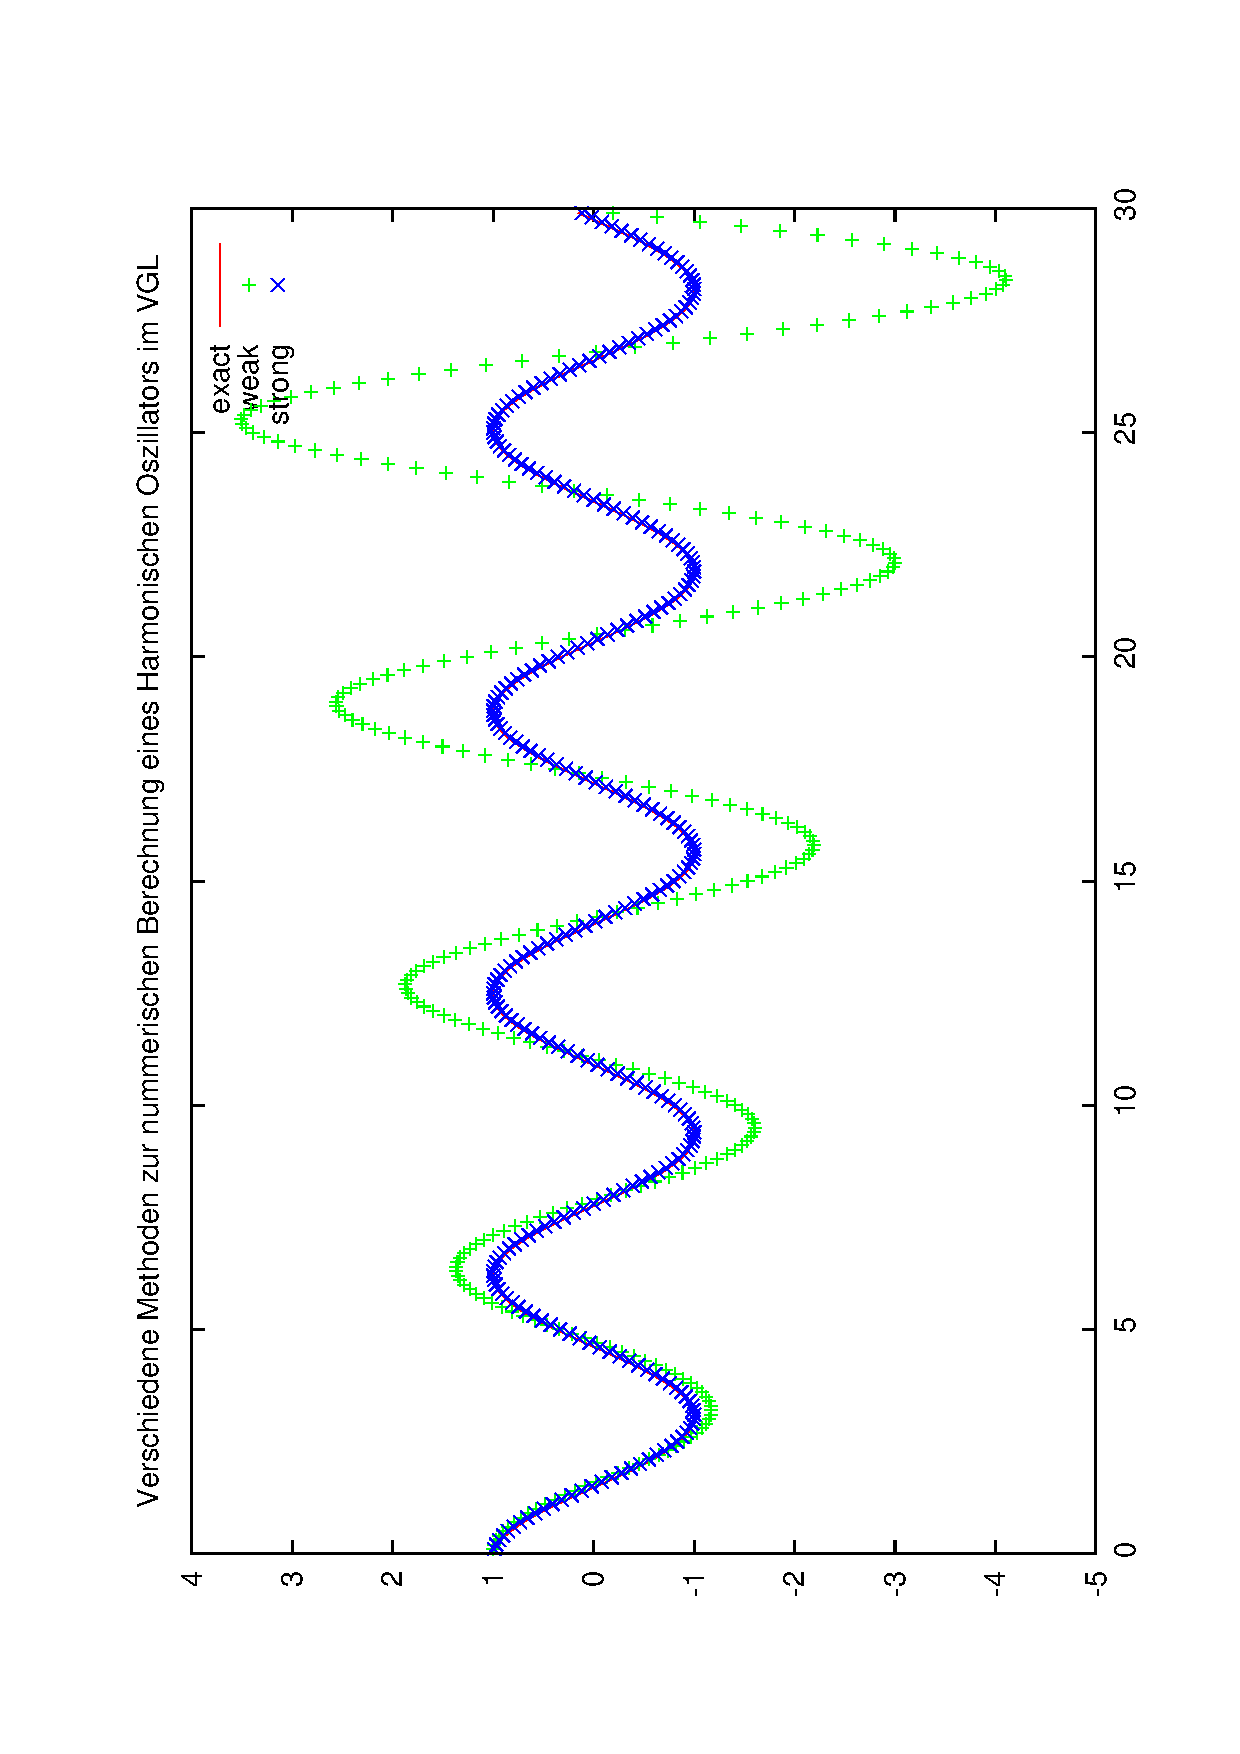
\includegraphics[angle=-90,width=0.48\textwidth]{bilder/my_harmon01-1}}
\subfigure[Im Kleinen]{\includegraphics[angle=-90,width=0.48\textwidth]{bilder/my_harmon01-2}}
  \caption{Vergleich von starkem und schwachen Algorithmus}
  \label{fig:vergleich_harmon_strong_weak}
\end{figure}


Um die "`starke"' Version zu erstellen verwendet man in dem
Gleichungssystem anstatt $v(s)$ auf der rechten Seite untenein
$v(s+\Delta s)$. Dieses Gleichungssystem
\begin{equation}
\label{eq:17}
  \begin{aligned}
      v(s+\Delta s) \approx v(s) - C \cdot u(s) \cdot \Delta s \\
      u(s + \Delta s) \approx u(s) + v(s+\Delta s) \cdot \Delta s
  \end{aligned} 
\tag{1.27}
\end{equation}
enth"alt die Energieerhaltung besser\footnote{dazu sp"ater mehr} und
liefert deshalb bessere Ergebnisse.







\subsection{Implementierung}
\label{sec:implementierung}

Vergleiche Listing \ref{my_harmon01}.



\lstinputlisting[firstline=14,label=my_harmon01,caption=Simulation
Harmonischer Oszillator]{./code/my_harmon01.cpp} 








\chapter{Interpolieren}
\label{sec:interpolieren}


Im Allgemeinen geht es bei Interpolieren und Approximieren darum, eine
Funktion $f$ oder Datenpunkte $(x_i, y_i)$ durch eien Funktion $g$ zu
approximieren, sodass $\|f-g\|$ bzw. $\|g(x_i) - y_i\|$ minimal wird.

Man unterscheidet zwischen {Interpolieren} und
{Approximieren}: Beim \textbf{Approximieren} N"ahert man eine
Funktion so an, dass sie eine Punktwolke m"oglichst gut beschreibt --
das bedeutet, dass die Summe der Quadrate der Abweichungen minimal
wird. Die schlie"slich gefundene Funktion l"auft an vielen
Funktionswerten vorbei. Beim \textbf{Interpolieren} jedoch findet man
ein Funktion, die die Menge von Punkten \emph{enth"alt} -- also durch
jeden einzelnen der vorgegebenen Punkte geht.

Es macht also Sinn, viele Messwerte, die von sich aus mit Fehlern
(Messfehlern usw) behaftet sind, durch eine Funktion
\emph{approximieren}, wohingegen man bei nur sehr d"unn gestreuten
Punkten eher \emph{interpoliert}.

Eine typische Aufgabe der Interpolation besteht darin, ein Polynom der
Ordnung $n$ durch $n+1$ St"utzstellen zu legen, sodass also
\begin{equation}
  \label{eq:26}
  P_n(x_i) = y_i \text{ f"ur } i \in \{0,...,n\}
\end{equation}
gilt. 
\begin{Wichtig}
  Dieses Polynom ist eindeutig.
\end{Wichtig}

Die Punkte $(x_i,y_i)$ k"onnen dabei beispielsweise von einer zu
approximierenden Funktion $f$ stammen: $y_i = f(x_i)$.


\section{St"utzstellen}
\label{sec:stutzstellen}

M"ochte man die Funktion $f$ durch ein Polynom $P_n$ approximieren, so
ben"otigt man die St"utzstellen $x_i$, an denen die Punkte $(x_i,y_i)$
als Grundlage verwendet werden sollen. Eine einfache Wahl der
St"utzstellen ist die \emph{"aquidistante}; im Intervall $[a,b]$ liefert
\begin{equation}
  \label{eq:27}
  x_i = a + \frac{b-a}{n} \cdot i ~ \;, i \in \{0,...,n\} 
\end{equation}
$n+1$ St"utzstellen.

Bei dieser Wahl wird jedoch der Fehler der approximierenden Polynome
am Rand von $[a,b]$ sehr gro"s. Um dem entgegenzusteuern
verwendet man die \emph{Tschebyscheff-Punkte}:
\begin{equation}
  \label{eq:28}
  x_i = \frac{a+b}{2} + \frac{a-b}{2} \cos\left ( \frac{i}{n} \pi
  \right ) ~\;, i \in \{0,...,n\} \;.
\end{equation}





\section{Lagrange-Interpolation}
\label{sec:lagrange_interpolation}

Eine sch"one M"oglichkeit zur Interpolation stammt von Lagrange; bei
ihr verwendet man die \emph{Lagrange-Polynome}
\begin{equation}
  \label{eq:29}
  L_i(x) := \prod_{\stackrel{j = 0}{j \neq i}} ^n \frac{(x-x_j)}{(x_i
    - x_j)} \;.
\end{equation}
Diese haben die praktische Eigenschaft
\begin{equation}
  \label{eq:30}
  L_i(x_j) = \delta_{ij} \;.
\end{equation}

Damit f"allt es auch leicht, die Bedingung \eqref{eq:26}
zufriedenzustellen:
\begin{equation}
  \label{eq:31}
  P_n(x) = \sum_{i = 0}^n y_i L_i \;.
\end{equation}

Aufgeschrieben sieht das sch"on aus -- nur zum Programmieren ist es
weniger angenehm. 

Hier k"onnen wir jedoch schon ein Beispiel geben, wie die
Tschebyscheff-St"utzstellen die Fehler am Rand verkleinern; betrachte
dazu die Abbildungen \ref{fig:lagrange-interp}. Der Quellcode zu
diesen Abbildungen ist in Listing \ref{interp-lagrange}.

\begin{figure}
  \centering
  \subfigure{\includegraphics[width=0.45\textwidth]{./bilder/lagrange_n30_cosexp-1.eps}}
  \subfigure{\includegraphics[width=0.45\textwidth]{./bilder/lagrange_n30_expx2-1.eps}}
  \caption{Lagrange-Interpolation}
  \label{fig:lagrange-interp}
\end{figure}

\lstinputlisting[label=interp-lagrange,caption=Lagrange-Interpolation
mit Tschebyscheff und "aquidistanten
St"utzstellen]{./code/interp-lagrange01.cpp}




\section{Newton-Interpolation}
\label{sec:newton_interpolation}

Die Newton-Interpolation setzt auf eine andere Darstellung des --
eindeutigen -- Polynoms $P_n$:
\begin{equation}
  \label{eq:32}
  P_n(x) = \sum_{i=0} c_i \prod_{j = 0}^{i-1} (x-x_j) = c_0 +
  c_1(x-x_0) + c_2 (x-x_0)(x-x_1) + ... \;.
\end{equation}
Diese Darstellung hat den Vorteil, dass f"ur $x = x_k$ alle Summanden
ab Ordnung $k$ wegfallen: $P_n(x_0) = c_0$ oder $P_n(x_1) = c_0 +
c_1(x_1-x_0)$.
Auf diese Weise kann man sukzessive mit Bedingunge \eqref{eq:26} die
Koeffizienten ausrechnen. 

Es zeigt sich dabei, dass man diese Koeffizienten elegant ausrechnen
kann; die Methode hierzu hei"st "`Schema der dividierten
Differenzen"'. Sie beruht auf dem Zusammenhang
\begin{equation}
  \label{eq:33}
  c_i =: [x_0, ..., x_i] \;,
\end{equation}
wobei der Term $[x_0, ..., x_i]$ rekursiv definiert ist via
\begin{equation}
  \label{eq:34}
  [x_i, ..., x_j] = \frac{[x_i, ..., x_{j-1}] - [x_{i+1}, ...,
    x_j]}{x_i - x_j} ~ \text{ und } ~ [x_i] = y_i \;.
\end{equation}
So kann man aus den St"utzstellen die Differenzen 0. Ordnung ($[x_i]$)
erhalten und aus zwei davon die n"achster Ordnung. usw.

\abs
Auch die \emph{Auswertung} der so entstehenden Polynome ist relativ
einfach machbar: "Uber das \emph{Horner-Schema}; m"ochte man den
Funktionswert $P_n(\xi)$ wissen und kennt alle Koeffizienten $c_i$, so
kann man folgenden Algorithmus verwenden:
\begin{lstlisting}[caption=Horner-Schema,language=c++]{Horner-Schema}
double p = c[n];
for (int k = n-1; k >= 0; k--)
     p = c[k] + (xi - x[k]) * p;
\end{lstlisting}
Das gesuchte Ergebnis ist dann in \lstinline|p|, die St"utzstellen
$x_i$ sind hier \lstinline|x[i]|.









\section{Hermite-Interpolation}
\label{sec:hermite_interpolation}

Die Hermite-Interpolation ist eine Erweiterung der
Newton-Interpolation: Sind zus"atzlich zu den Werten der St"utzstelle
noch die \emph{Werte der Ableitung} an den Stellen gegeben -- also
neben $(x_i, y_i)$ noch $(x_i, y'_i)$ -- so kann man das obige Schema
erweitern: Das approximierende Polynom hat dann die Gestalt
\begin{equation}
  \label{eq:36}
  P_{2n+1}(x) = c_0 + c_1(x-x_0) + c_2 (x-x_0)^2 + c_3(x-x_0)^2(x-x_1)
  + ... \;,
\end{equation}
wobei das Schema zur Bestimmung der Koeffizienten sich so "andet, dass
sich vor der ersten Ordnung noch eien Reihe von Dividierten
Differenzen ergeben: $[x_i, x_i]$. Diese sind nach Definition
\eqref{eq:34} und ein
wenig Limesvertauschung so zu verstehen:
\begin{equation}
  \label{eq:35}
  [x_i, x_i] = \lim_{h\to 0}\frac{[x_i +h] - [x_i]}{x_i+h-x_i} =
  \lim_{h\to 0}\frac{f(x_i+h)-f(x_i)}{h} = f'(x_i) =: y'_i \;.
\end{equation}

Die Koeffizienten $c_i$ sind dann gegeben durch
\begin{equation}
  \label{eq:37}
  c_0 = y_0, c_1  = [x_0, x_0] = y_0', c_2 = [x_0,x_0,x_1], c_3 =
  [x_0,x_0,x_1,x_1], ... \;.
\end{equation}

Dieses Verfahren macht aber nur dann Sinn, wenn neben den
Funktionswerten auch die Ableitungswerte gegeben sind...






\section{Rationale Approximation}
\label{sec:rationale_approximation}

Approximiert man mit Polynomen, so hat man bei Funktionen mit
Polstellen ziemliche Probleme; hier werden die Approximationen
ziemlich schlecht. Um $n$ Punkte zu approximieren, verwendet man
deshalb die Rationale Funktion
\begin{equation}
  \label{eq:96}
  R(x) = \frac{p_0 + p_1 x^1 + ... + p_\mu x^\mu}{1 + 1_1 x^1 + ... +
    q_\nu x^\nu} ~ \text{ mit } \mu + \nu = n-1 \;.
\end{equation}

F"ur die $n$-Gleichungen $R(x_i) = y_i$ existiert stets eine L"osung,
nur leider kann diese ziemlich schlechte Ergebnisse liefern --
bspw. wenn Z"ahler und Nenner gleiche Nullstellen haben etc. In
solchen F"allen muss man die Interpolation mehrmals mit verschieder
Wahl von $(\mu,\nu)$ machen...

In der Praxis teilt man die zu approximierenden Punkte in Untermengen
mit nur wenigen St"utzstellen auf, die man dann einzeln interpoliert
und anschlie"send zusammensetzt. Die so entstandene Interpolation ist
i.A. "`nur"' stetig: Am Rand der Intervalle ergeben sich manchmal
Oszillationen, die die Differenzierbarkeit v"ollig unm"oglich machen.




\section{Splines}
\label{sec:splines}







\section{Numerisches Differenzieren}
\label{sec:numerisches_differenzieren}


Um eine Funktion zu differenzieren, n"ahern wir sie durch ein Polynom
an und differenzieren dieses. Das Verfahren, wie man auf dieses
Polynom kommt, ist nicht entscheidend, da das entstehende Polynom ja
eindeutig ist -- also bekommt man "uber andere Verfahren nur andere
Darstellungen des selben Polynoms.  Wir verwenden hier die
Lagrange-Interpolation (vgl. Kap \ref{sec:lagrange_interpolation}) und
au"serdem "aquidistante St"utzstellen -- das vereinfacht das Rechnen.

\abs
Um eine $n$-te Ableitung zu bestimmen, kann man die Funktion durch ein
Polynom $n$-ten Grades approximieren. Wenn dieses $n$-mal abgeleitet
wird, so hat man eine Konstante -- gesuchte Ableitung eben.

Verwendet man die Vereinfachung $\lambda_i = \left [ \prod_{j = 0; j \neq
  i}^n (x_i - x_j) \right ]^{-1}$, so gilt f"ur die $n$-te Ableitung
des Lagrange-Polynoms $P_n$:
\begin{equation}
  \label{eq:38}
  \frac{\diff ^n}{\diff x^n} P_n(x) = \sum_{i = 0}^n \, y_i \lambda_i
  \, n! \approx f^{(n)}(x) \;.
\end{equation}
Verwendet man die "Aquidistanz der St"utzstellen -- alle haben den
Abstand $h$ voneinander --, kann man den
Ausdruck $\lambda_i$ noch vereinfachen: $\lambda_i = \binom{n}{i}
\cdot \left [ (-1)^{n-i} \, h^n \, n! \right ]^{-1}$. F"ur die
Ableitung kommt man dann auf
\begin{equation}
  \label{eq:39}
  \frac{\diff ^n}{\diff x^n}P_n(x) = 
  \frac{1}{h^n}\sum_{i=0}^n \binom n i (-1)^{n-i}y_i 
% =
% \frac{1}{h^n} \left [ (-1)^ny_0 +
%     (-1)^{n-1} \binom{n}{1}y_1 \right ]
\;.
\end{equation}

F"ur den Spezialfall $n=1$ hat man damit die einfachste Numerische
Ableitung:
\begin{equation*}
  f'(x) \approx \frac{1}{h} (y_1 - y_0) = \frac{f(x+h) - f(x)}{h} \;,
\end{equation*}
f"ur $n=2$ 
\begin{equation*}
  f''(x) \approx \frac{1}{h^2} (y_2 - 2y_1 + y_0) = 
\frac{ \frac{y_0 - y_1}{h} - \frac{y_1 - y_2}{h} }{h} 
\end{equation*}
usw.

Dies Art der Approximation ist aber nicht besonders genau -- es ist
sogar die schlechteste, die gerade noch so den Job tun kann.

\abs
Bessere Approximationen bekommt man, wenn man f"ur die Bildung einer
$k$-ten Ableitung ein Polynom der Ordnung $n > k$ verwendet. Ein
entscheidender Unterschied zum obigen Fall ist der, dass hier die
Ableitung keine konstante Funktion mehr ergibt -- man muss also darauf
achten, an welcher Stelle man das abgeleitete Polynom
\emph{auswertet}.

Nach der Bildungsvorschrift aus Kap. \ref{sec:lagrange_interpolation}
k"onnen wir bspw. das Polynom $P_2$ aufschreiben -- wobei wir wieder
die "Aquidistanz ausnutzen --:\footnote{Bemerkung: Das "`$-$"' vor dem
zweiten Summanden kommt daher, dass der Nenner eigentlich negativ ist.}
\begin{equation*}
  P_2(x) = \frac{y_0 (x-x_1)(x-x_2)}{2h^2} 
- \frac{y_1 (x-x_0)(x-x_2)}{h^2} 
+ \frac{y_2 (x-x_0)(x-x_1)}{2h^2} \;.
\end{equation*}
Leitet man diesen Term an der Stelle $x_1$ ab, erh"alt man 
$$P'_n(x_1) = {{\left({ x_1}-{ x_0}\right)\,{ y_2}+\left(2\,{ x_2}-4
 \,{ x_1}+2\,{ x_0}\right)\,{ y_1}+\left({ x_1}-{ x_2}
 \right)\,{ y_0}}\over{2\,h^2}} =
\frac{+y_2 - y_0}{2h} \;,
$$
was schon eine bessere Approximation ist. Analog kann man noch mit
einem Polynom dritter Ordnung approximieren und ableiten und erh"alt
immer bessere Ableitungen. Vergleiche dazu Abb. \ref{fig:vlg-abl}.

\begin{figure}
  \centering
  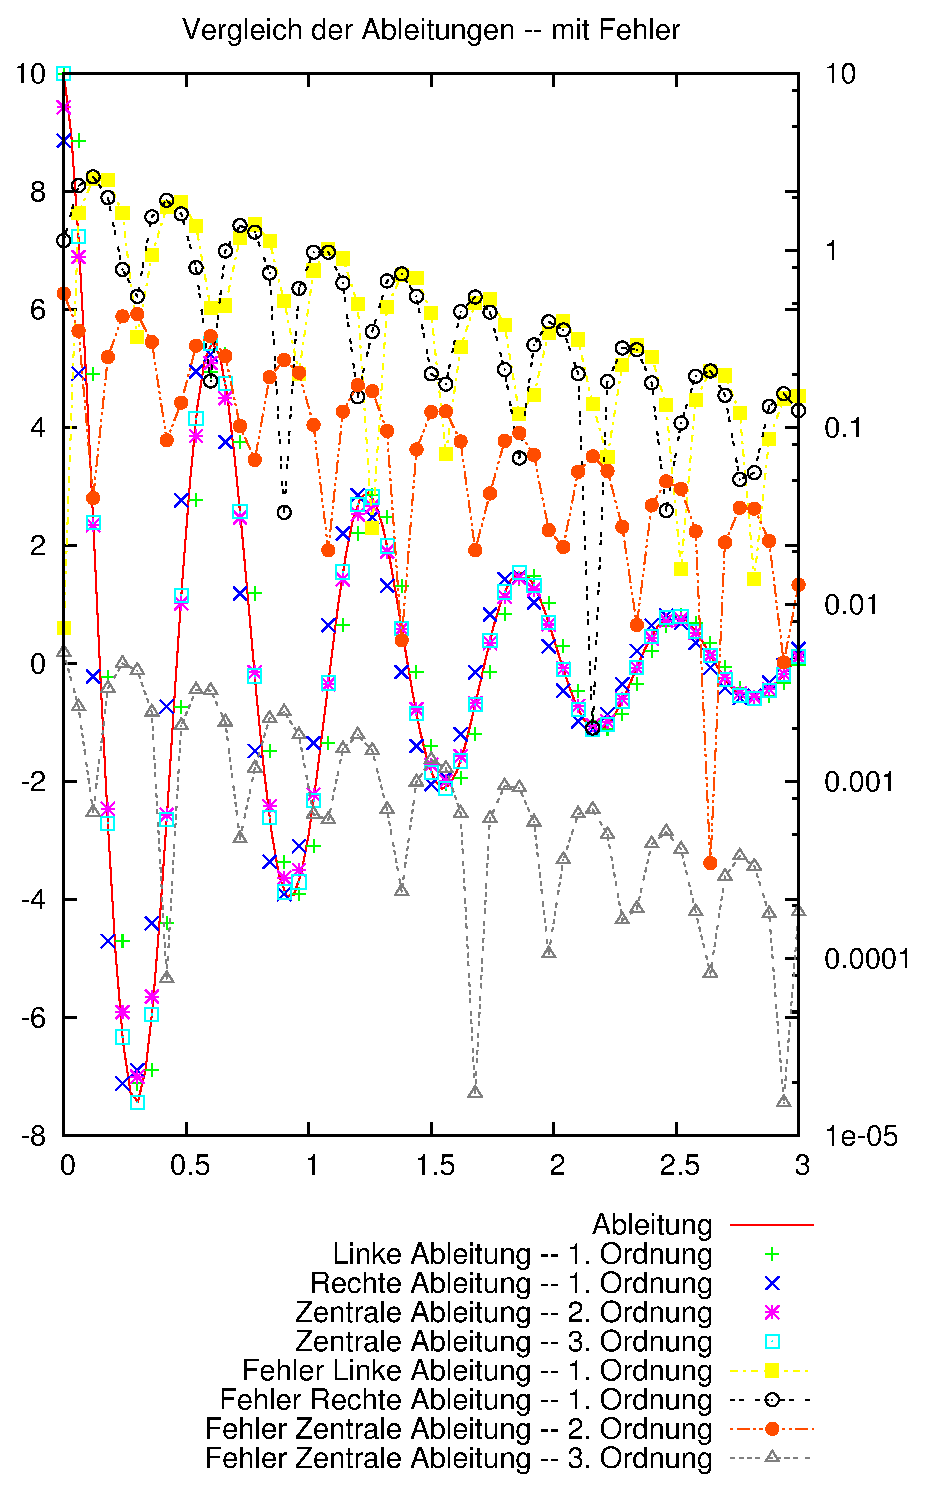
\includegraphics[width=\textwidth, height=0.7\textheight]{./bilder/vgl-abl}
  \caption{Vergleich verschiedener (erster) Ableitungen mit Fehler}
  \label{fig:vlg-abl}
\end{figure}

Auf die gleiche Art und weise kann man nat"urlich auch h"ohere
Ableitungen berechnen. Hier noch Approximation in 3. Ordnung:

\begin{align*}
  f'(\bar x) \approx& \frac{1}{24h} (y_0 - 27y_1 + 27y_2 - y_3) \text{ wobei
  } \bar x = \frac{1}{2}(x_0 + x_3) \;, \\
  f''(\bar x) \approx& \frac{1}{2h^2} (y_0 - y_1 -y_2 + y_3 ) \;.
\end{align*}







\section{Auswertung an bestimmter Stelle}
\label{sec:ausw_an_best_stell}


\subsection{Neville-Schema}
\label{sec:neville_schema}


Sind St"utzstellen $(x_i,y_i)$ mit $i \in \{ 0, ..., n\}$ gegeben und
man m"ochte f"ur einen bestimmten Punkt $\xi$ den Interpolierten Wert
wissen, so verwendet man die folgende Rekursionsbeziehung:
F"ur diejenigen eindeutigen Polynome $P_{j,
  j+1, ..., j+m}$ mit $j+m \leq m$, welche $P_{j, ..., j+m}(x_i) =
y_i$ f"ur $i \in \{j, ..., j+m\}$ erf"ullen, gilt
\begin{equation}
  \label{eq:94}
  P_{j,...,j+m}(x) = \frac{(x-x_j)P_{j+1,...,j+m}(x) -
    (x-x_{j+m})P_{j,...,j+m-1}(x)}{x_{j+m} - x_j}
\end{equation}
wenn man
\begin{equation}
  \label{eq:95}
  P_j(x) : \equiv y_j
\end{equation}
setzt. 

M"ochte man nun also den Wert $f(\xi)$ interpolieren, berechnet man
nacheinander (f"ur festes $\xi$) die immer h"oheren Polynome
$\left. P_{...} \right|_{x = \xi}$ und setzt sie weiter zusammen.






\subsection{Extrapolation}
\label{sec:extrapolation}


Um \emph{noch} genauere Ergebnisse f"ur die Funktionsauswertung
bzw. Ableitungen zu erhalten, kann man wie folgt vorgehen: Mit der
Schrittweite $h$ berechnet man einen N"aherungswert $\eta^h$ der
gesuchten Gr"o"se. Dann variiert man das $h$ -- man bildet eine Folge
$(h_j)_j$, sodass $h_{j+1} < h_j$, mit ein paar Gliedern und
interpoliert dann die Messpunkte $(h_j, \eta^{h_j})$ mit einem der
oben genannten Verfahren. In der Interpolation untersucht man dann
$h=0$.



\section{Gau"s-Approximation}
\label{sec:gaus_approximation}

Die Gau"s Approximation unterscheidet sich im Grundsatz nicht
besonders von den bisher angesprochenen Methoden; Eine Funktion $f$
soll durch $g$ so approximiert werden, dass $\|f-g\|$ minimal
ist. Wenn $\|\cdot\|$ minimal sein soll, ist das gleichbedeutend
damit, dass $\|\cdot\|^2 = \langle \cdot \,|\,\cdot  \rangle$ minimal
sein soll.

In dem zur Approximation zur Verf"ugung stehenden Raum $U$ seien die
linear unabh"angingen Funktionen $\{\varphi_i\}_i$ gegeben -- es ist
also automatisch $U = \operatorname{span}(\varphi_0,\varphi_1, ..., \varphi_n)$
-- , dann ist
\begin{equation*}
  g = \alpha^i \varphi_i \;.
\end{equation*}
Die beste Approximation von $f$ in $U$ -- wobei $f$ nat"urlich nicht
unbedingt in $U$ liegen muss -- ist erreicht, wenn $\langle \varphi_i
\,|\, f-g  \rangle = 0$ $\forall i$, denn dann verschwindet die Projektion von
$f-g$ nach $U$. Mit der Darstellung von $g$ kann man dies umschreiben:
\begin{equation}
  \label{eq:40}
  \langle \varphi_i \,|\, f \rangle - \langle \varphi_i \,|\,g\rangle
  = 0 \gdw
\langle \varphi_i \,|\, f \rangle = \langle \varphi_i \,|\, \varphi_j
\rangle \alpha^j \;.
\end{equation}
Und das wiederum ist ein Matrix-Gleichungssystem:
\begin{equation*}
  \vec f = \Mat A \cdot \vec \alpha \;,
\end{equation*}
wobei $\det\Mat A \neq 0$ ist, weil die $\varphi_i$ linear unabh"angig
sind. Damit existiert $\Mat A^{-1}$ und damit eine eindeutige L"osung
f"ur die $\alpha^i$, n"amlich
\begin{equation*}
  \vec \alpha = \Mat A^{-1} \cdot \vec f \;.
\end{equation*}



\subsection{Diskrete Gau"s-Approximation}
\label{sec:diskrete_gaus_approximation}

Hat man eine Datenmenge $(x_i, f_i)$ vorliegen, so ist das
Skalarprodukt der Wahl
\begin{equation}
  \label{eq:41}
  \langle u \,|\, v \rangle = \sum_{i} u(x_i) \, v(x_i) \, \omega(x_i) \;,
\end{equation}
wobei $\omega$ eine Gewichtungsfunktion ist.


\subsection{Kontinuierliche Gau"s-Approximation}
\label{sec:kontinuierliche_gaus_approximation}

Der Raum $U$, in dem approximiert werden soll, ist jetzt der Raum der
quadratintegrablen Funktionen $L_2([a,b])$ und das Skalarprodukt ist 
\begin{equation}
  \label{eq:42}
  \langle u \,|\,v  \rangle = \int_{a}^b u(x)\,v(x)\,\omega(x)\diff x 
\end{equation}
und $\omega$ ist wieder eine (integrierbare) Gewichtungsfunktion.

Um das zu l"osende Gleichungssystem \eqref{eq:40} besser l"osen zu
k"onnen, verwendet man als Basis in $U=L_2$ ein System
\emph{orthogonaler} Funktionen (also $\langle \varphi_i \,|\,\varphi_j
\rangle \propto \delta_{ij}$) -- damit hat die Matrix $\Mat A$ nur
noch Eintr"age auf ihrer Diagonalen und es gilt einfach
\begin{equation}
  \label{eq:43}
  \alpha^i = \frac{\langle \varphi_i \,|\, f \rangle}{\langle
    \varphi_i \,|\,\varphi_i  \rangle} \;.
\end{equation}




\subsubsection{Trigonometrische Approximation}
\label{sec:trigonometrische_approximation}

Die Funktionen
\begin{equation}
  \label{eq:44}
  \sin(i x) \text{ und } \cos(ix) \text{ mit } i \in \{0, ..., n\}
\end{equation}
sind auf $[-\pi,\pi]$ orthogonal. Enwickelt (bzw. approximiert) man $f$
mit diesen kommt das eine Fourierreihenentwicklung gleich.

Diese l"asst sich mit der \emph{fast fourier transformation}
"okonomisch berechnen.




\subsubsection{Tschebuscheff-Polynome}
\label{sec:tschebuscheff_polynome}

Grundlage f"ur diese Orthogonalen Polynome sind die Additionstheoreme
des Cosinus; mit diesen ist $\cos( n \varphi)$ als Polynom vom Grad $n$
in $\cos \varphi$ darstellbar.

Entsprechend zu \ref{sec:trigonometrische_approximation} sind die
Tschebyscheff-Polynome:
\begin{equation}
  \label{eq:45}
  T_n(x) = T_n(\cos \varphi) = \cos(n \, \varphi) \text{ ~ und } x \in
  [-1,1] \;.
\end{equation}
Um wirklich $T_n(x)$ zu erhalten, verwendet man\footnote{Vgl Bronstein}\begin{align}
  \label{eq:46}
  \cos(n\varphi) = 
\cos^n\varphi
- \binom n 2 \cos^{n-2}\varphi\sin^2\varphi
+ \binom n 4 \cos^{n-4}\varphi\sin^4\varphi \\
- \binom n 6 \cos^{n-6}\varphi\sin^6\varphi
+ \dots \;;
 \nonumber
\end{align}
mit der Substitution
\begin{equation}
  \label{eq:47}
  \cos\varphi = x \text{ und } \sin\varphi = \sqrt{1-x^2} \;.
\end{equation}

Es gilt die Rekursionsformel
\begin{equation*}
  T_{n_1} = 2x \, T_n - T_{n-1} \text{ f"ur } n \geq 1 \text{ und }
  T_0(x) = 1, T_1(x) = x \;,
\end{equation*}
sowie die Beziehungen
\begin{align*}
  T_n(-x) &= (-1)^n T_n(x) \\
  | T_n(x) | &\leq 1 \\
  T_n(x) &= 2^{n-1}x^n + \dots \text{ (f"uhrender Koeff: } 2^{n-1}
  \text{ ). }
\end{align*}


F"ur das Skalarprodukt\footnote{Der Term $\omega(x) = 1/\sqrt{1-x^2}$
  ist formal eine Gewichtungsfunktion.}
\begin{equation*}
  \langle u \,|\, v \rangle = \int_{-1}^1
  u(x)\,v(x)\,\frac{1}{\sqrt{1-x^2}} \diff x
\end{equation*}
sind die Polynome \emph{orthogonal}:\footnote{Das sieht man leicht,
  weil $1/sqrt{1-x^2} = 1/\sin x$ ist und $\diff(\cos x) = -\sin x
  \diff x$, womit man wieder die Trigonometrischen Funktionen von
  vorher hat.}
\begin{equation*}
  \langle T_k \,|\,T_j  \rangle =
  \begin{cases}
     \frac{\pi}{2} \delta_{kj} & k=j\neq 0\\
     \pi & k = j = 0 
  \end{cases} \;.
\end{equation*}

Die Approximierende Funktion $g$ -- ein Polynom der Ordnung $n$ --
stellt man mit den Polynomen $T_k$ dar via
\begin{equation}
\label{eq:48}
  g_n = \frac{c_0}{2}T_0 + \sum_{k=1}^n c_k T_k \text{ mit } c_k =
  \frac{2}{\pi} \int_{-1}^1 f(x) T_k(x) \frac{1}{\sqrt{1-x^2}} \diff x \;.
\end{equation}
Mit Symmetrien\footnote{bspw des Cosinus} und der
Fouriertransformation\footnote{die hier nicht besprochen wird} erh"alt
man als N"aherung
\begin{equation}
  \label{eq:49}
  c_k \approx \frac{2}{n} \left ( 
    \frac{1}{2}\left ( f(1) + f(-1)\cos(\pi k) \right )
    +
    \sum_{j=1}^{n-1} f(\cos \left(\frac{j}{m} \pi\right) ) \cdot
    \cos(\frac{j}{m}k\pi) 
 \right ) \;,
\end{equation}
wobei man den Fehler absch"atzen kann durch
\begin{equation*}
  \|f-g_n\| \leq _{k = n+1}^\infty |c_k| \;.
\end{equation*}

Mit dem \emph{Algorithmus von \textsc{Clenshaw}} kann man die
Auswertung von $g_n$ an einer Stelle $x$ effizient programmieren:
\begin{lstlisting}[language=c++]
d[n] = c[n];
y = 2 * x;
d[n-1] = c[n-1] + y * c[n];
for(int k = n-2; k >= 0; k--)
{
     d[k] = c[k] + y * d[k+1]-d[k+2];
}
gn = (d[0] - d[2]) / 2.0;
\end{lstlisting}



\abs
M"ochte man eine Menge von $n$ Punkten $(x_i,y_i)$ mit den
Tschebyscheff-Polynomen approximieren, sodass also $g_n(x_i) = y_i$
gilt, dann gilt f"ur das $g_n$ aus \eqref{eq:48} mit dem
"`Skalarprodukt"'
\begin{equation*}
  \sum_{l=1}^{n+1} T_k(x_l) T_j(x_l) = 
  \begin{cases}
    0 & k \neq j \\
    (n+1)/2 & k = j \neq 0 \\
    n+1 & k=j=0 
  \end{cases} \;;
\end{equation*}
daf"ur m"ussen aber $x_l$ die Nullstellen von $T_{n+1}$ sein:
\begin{equation*}
  x_l = \cos( \frac{(2l-1)}{(n+1)} \, \frac{\pi}{2} ) \;,
\end{equation*}
dann erh"alt man f"ur die Koeffizienten 
\begin{equation}
  \label{eq:50}
  c_k = \frac{2}{n+1} \sum_{l=1}^{n+1} f( x_l ) \, \cos( k \, x_l ) \;.
\end{equation}





\subsubsection{Legender-Polynome}
\label{sec:legender_polynome}


Die Legender-Polynome sind definiert als
\begin{equation}
  \label{eq:51}
  P_n(x) = \frac{1}{2^n \, n!} \, \frac{\diff ^n}{\diff x^n} \left (
    (x^2 - 1)^n \right ) \;,
\end{equation}
und sind \emph{orthogonal} unter dem Skalarprodukt\footnote{Hier ist
  -- formal -- die oben angesprochene Gewichtungsfunktion $\omega(x)
  \equiv 1$.}
\begin{equation}
  \label{eq:52}
\langle u \,|\, v \rangle = \int_{-1}^1
  u(x)\,v(x) \diff x \;;
\end{equation}
mit
\begin{equation}
  \label{eq:53}
  \langle P_k \,|\, P_l  \rangle = \frac{2}{2n+1} \, \delta_{kl} \;.
\end{equation}

Das Legendrepolynom $P_n$ hat die Ordnung $n$ und im Intervall
$[-1,1]$ $n$ \emph{einfache Nullstellen}, und es gilt die Rekursion
\begin{equation}
  \label{eq:54}
  P_{n+1} = \frac{2n+1}{n+1} \, x\, P_n - \frac{n}{n+1} \, P_n \text{
    f"ur } n \in \{1,2,...\} \text{ und } P_o(x) =1 \text{ und }
  P_1(x) = x \;.
\end{equation}
Auf f"ur sie gilt die Eigenschaft $| P_n (x) | \leq 1$ f"ur $x \in
[-1,1]$.

Das N"ahrungspolynom $g_n$ der Ordnung $n$ stellt man dar mit
\begin{equation}
  \label{eq:55}
  g_n = \sum_{k=0}^n c_k P_k \text{ mit } c_k = \frac{1k+1}{2}
  \int_{-1}^1 f(x) \, P_k(x) \diff x \;.
\end{equation}
Hier muss man jedoch die Koeffizienten ausrechnen -- mit Methoden wie
sie weiter unten besprochen werden: N"aherungsweise mit der
\emph{Gau"s-Quadratur}.






















\chapter{Numerisches Integrieren}
\label{sec:numer_integr}


Allgemein versucht man, das bestimmte Integral $\int_a^b f(x) \diff x$
durch eine Summe anzun"ahern:
\begin{equation}
  \label{eq:56}
  \int_a^b f(x) \diff x \approx \sum_{i=0}^n w_i f(x_i) \;.
\end{equation}
Die $w_i$ hei"sen (Integrations)\emph{Gewichte} und die $x_i$ hei"sen
\emph{St"utzstellen}. Die Wahl von $w_i$ und $x_i$ werden durch die
jeweilige Integrationsregel festgelegt.

\abs
Man Spricht von einem \textbf{Genauigkeitsgrad } $m$, wenn \eqref{eq:56}
eine \emph{Gleich}ung ist mit einem Polynom $f$ mit
$\operatorname{grad} f \leq m$: Ein Polynom bis zum Grad $m$ wird
exakt approximiert.



\section{Newton-Cotez}
\label{sec:newton_cotez}


Mit $n+1$ St"utzstellen $x_0, ..., x_n$ wir die Funktion $f$ mit Lagrange Interpoliert
(vgl Kap. \ref{sec:lagrange_interpolation}) und das Polynom integriert:
\begin{equation}
  \label{eq:57}
  \int_a^b f(x) \diff x \approx 
\int_a^b \sum_{i=0}^n f(x_i) L_i(x) \diff x
=
 \sum_{i=0}^n f(x_i) \underbrace{\int_a^b L_i(x) \diff x}_{w_i} \;.
\end{equation}
Die St"utzstellen kann man der Einfachheit halber "aquidistant
w"ahlen.

F"ur $n=1$ erh"alt man so
\begin{equation*}
  P_1(x) = f(x_0)\frac{x-x_1}{x_0-x_1} + f(x_1)\frac{x-x_0}{x_1-x_0} = 
f(x_0)\frac{x-x_1}{-h} + f(x_1)\frac{x-x_0}{h}
\end{equation*}
und Integration mit den Grenzen $a = x_0$ und $b = x_1$ liefert die
\textbf{Trapezregel}
\begin{equation}
  \label{eq:58}
  \int_{x_0}^{x_1} f(x) \diff x  \approx (x_1-x_0) \, \frac{y_0 + h_1}{2} \;.
\end{equation}
Analog kann man mit $n=3$ vorgehen; setzt man als St"utzstellen $x_0 =
a$, $x_1 = \frac{a+b}{2}$ und $x_2 = b$ so folgt die
\textbf{Simpsonregel}
\begin{equation}
  \label{eq:59}
  \int_{x_0}^{x_2} f(x) \diff x \approx 
(x_2-x_0) \frac{f(x_0) + 4 f(x_1) + f(x_2)}{6} \;.
\end{equation}

\abs
Diese Algorithmen sind jedoch nur f"ur kleine $n$ stabil. Um eine
h"ohere Genauigkeit f"ur das approximierte Integral zu bekommen, macht
es eshalb weniger Sinn, die Funktion $f$ durch h"ohere Polynome zu
approximieren, sondern vielmehr teilt man den Integrationsbereich
$[a,b]$ in viele kleien Unterbereiche auf, die man dann jeweils wieder
mit Trapez- oder Simpsonregel integriert.

F"ur die Trapezregel ergibt sich so beispielsweise, wenn man $[a,b]$
in $n$ Teilintervalle aufteilt:
\begin{equation}
  \label{eq:60}
  \int_a^b f(x) \diff x 
\approx
h \, \left ( \frac{y_0}{2} \sum_{i=1}^{n-1} + \frac{y_n}{2} \right ) \;.
\end{equation}

Die Methode eignet sich besonders f"ur periodische Funktionen mit der
Periode $[a,b]$.




\paragraph{Erstes adaptives Integrieren}
\label{sec:erstes_adaptives_integrieren}


Nun wollen wir ein Verfahren betrachten, wie die
Integartionsgenauigkeit gesteigert werden kann: Der Komputer soll in
der Lage sein, zu entscheiden, wie weit er das Intervall $[a,b]$
aufteilen soll. 

Dazu machen wir den -- etwas naiven -- Ansatz zur Integration, der
sich aus der Riemann'schen Theorie ergibt: Die
\textbf{Mittelpunktsregel}: Das Intervall $[a,b]$ wird in $n$ Teilintervalle
der Breite $h$ aufgeteilt und in der Mitte des Teilintervalls wird der
Funktionswert verwendet:
\begin{equation}
  \label{eq:61}
  \int_a^b f(x) \diff x \approx
\sum_{i=0}^{n-1} h \, y_{i+\frac{1}{2}}
\end{equation}

Bezeichnet man nun mit $T(h)$ die Trapezregel mit Schrittweite $h$ und
mit $M(h)$ die Mittelpunktsregel mit Schrittweite $h$, so sieht man
anhand \eqref{eq:60} und \eqref{eq:61}, dass
\begin{equation}
  \label{eq:62}
  \frac{M(h) + T(h)} 2 = T(\frac{h}{2}) \;,
\end{equation}
einfach weil die Randterme mit $y_0/2$ und $y_n/2$ vorkommen und jetzt
zwischen dei einzelnen Summanden von $T(h)$ die Summanden von $M(h)$
"`dazwischen geschoben werden"'. Damit man wieder eine Form wie
\eqref{eq:61} bekommt, muss man noch die Schrittweite anpassen, damit
zwischen $a$ und $b$ weiterhin $n$ Schritte passen: Die Schrittweite
wird halbiert.

Die Gl. \eqref{eq:62} kann man als Rekursionsbeziehung f"ur die
Verfeinerung der Trapezregel ansehen: Man berechnet $T(h)$ und $M(h)$
und wenn $|T(h) - M(h)| \geq \varepsilon$ ist (mit einer vorher fest
gew"ahlten Toleranz $\varepsilon$), dann bestimmt man mit den beiden
Integralen "uber \eqref{eq:62} $T(h/2)$ und anschlie"send $M(h/2)$. Um
"okonomisch vorzugehen kann man dabei verwenden, dass man bei $M(h/2)$
nur noch die H"alfte der Approximation neu berechnen muss: Jedes
zweite Teilintervall ist bereits in $M(h)/2$ eingegangen. So ben"otigt
man f"ur die Berechnung von $M(h/2)$ nur noch $n$ Rechenschritte. Dies
ist die Idee, der adaptiven Integration; vgl
Kap. \ref{sec:adaptive_integration}.

Die Idee dabei ist, dass wen zwei Approximationsmethoden beinahe das
selbe Ergebnis liefern, dass dann das \emph{tats"achliche} Ergebnis
nicht mehr zu stark abweichen darf/kann/sollte.

Bei abklingenden Funktionen kann man in den Algorithmus einbauen, dass
weitere Funktionswerte ab $f(x) \leq \delta$ (mit einem vorher
gew"ahlten $\delta$) verworfen werden.







\section{Rombert-Integration}
\label{sec:rombert_integration}

Eine weitere M"oglichkeit, die -- relativ einfache -- Trapezformel zu
verbessern ist ein Ansatz, in dem man die Fehlerentwicklung der
Approximationen f"ur verschiedene Schrittweiten $h$ so kombiniert,
dass in der entstehenden Entwicklung niedrige Ordnungen wegfallen. Im
Klartext: Kluge Menschen haben eine Formel entwickelt, nach der man
Trapezregeln mit verschiedenen Schrittweiten so miteinander verrechnen
kann, dass das Ergebnis noch genauer ist, weil sich bestimmte Fehler
gegenseitig wegheben.

Dazu definiert man f"ur die einfache Trapezregel
\begin{equation}
  \label{eq:63}
  T_{k,0} = T(h_k) \text{ wobei } h_k = \frac{b-a}{2^k} \text{ und } k
  \in \{0, ..., n\} \;,
\end{equation}
und weiter die Rekursion
\begin{equation}
  \label{eq:64}
  T_{k,j} = \frac{4^j \, T_{k,j-1} - T_{k-1,j-1}}{4^j - 1} \text{ mit
  } j \in \{1,2,...,n\} \text{ und } k \in \{ j, j+1, ..., n
\} \;.
\end{equation}
Diese definiert eine Dreiecksstruktur; bspw f"ur $n=3$:

\begin{tabular}{c c c c c c c r}
  & & & $T_{33}$ & & & & Exaktestes Ergebnis\\
  & & $T_{32}$ & & $T_{22}$ \\
   & $T_{31}$ & & $T_{21}$ & & $T_{11}$ & \\
  $T_{30}$ &   & $T_{20}$  & & $T_{10}$ & & $T_{00}$ & Trapezregeln
\end{tabular}

Mit den vier Trapezregeln in der untersten Zeile kann man die dar"uber
liegenden $T_{k,l}$-Werte mit geringem Aufwand berechnen und so eine
wesentlich genauere Approximation erhalten.


\paragraph{Wieder adaptiv integrieren}
\label{sec:wieder_adaptiv_integrieren}

M"ochte man hier wieder den Komputer entscheiden lassen, wie viele
Iterationsschritte m"oglich sind, so kann man sich an den Rechten Rand
der Dreiecksstruktur wenden: Man bestimmt $T_{0,0}$ und anschlie"send
$T_{1,1}$. Ist die Differenz der beiden Werte kleiner als eine
Toleranz $\varepsilon$, wird kein weiterer Wert berechnet, wenn nicht,
wird $T_{2,2}$ berechnet usw.








\section{Gau"s-Integration}
\label{sec:gaus_integration}

Die Gau"s-Integration greift auf die orthogonalen Legender-Polynome
zur"uck -- vgl. Kap. \ref{sec:legender_polynome}. Da diese nur auf dem
Intervall $[-1,1]$ ihre Wunscheigenschaften haben (also bspw. die
Orthogonalit"at), kann man f"ur diese Integration auch nur das
Intervall $[-1,1]$ verwenden. Durch die Lineare Transformation
\begin{equation}
  \label{eq:66}
  \Psi : [a,b] \to [-1,1]; ~ x \mapsto t = \frac{b-a}{2}x + \frac{a+b}{2}
\end{equation}
kann man dem jedoch abhelfen:
\begin{equation}
  \label{eq:67}
  \int_a^b f(x) \diff x =
\frac{b-a}{2} \int_{-1}^1 f(\frac{b-a}{2}x + \frac{a+b}{2}) \diff x
\end{equation}


\abs
Die Idee bei der Gau"s-Integration ist, dass sowohl die St"utzstellen
$x_i$ als auch die Integrationsgewicht $w_i$ so gew"ahlt werden
sollen, dass der \emph{Genauigkeitsgrad} der Integration m"oglichs
hoch ist -- also dass ein Polynom von m"oglichst hohem Grade noch
exakt berechnet werden kann. 

Bei der Gau"s-Integration l"asst sich dabei mit $n$ St"utzstellen
noche in Polynom vom Grad $2n-1$ exakt berechnen\footnote{Dass dies
  das \emph{Maximum} ist, kann man
zeigen, indem man ein Polynom $P_n$ vom Grade $2n$ konstruiert mit
$P_n(x) = \prod_{i=1}^n (x-x_i)^2$: Es ist $P(x) \geq 0$ und damit
auch sein Integral, f"ur jede St"utzstelle $x_i$ ist jedoch $P(x_i) =
0$ und damit verschwindet das approximierte Integral: Hier macht man
also einen Fehler.}, bei Newton-Cotez ist
geht es nur bis zu Polynomen der Ordnung $n-1$. Den "`Preis"', den man
daf"ur zahlen muss, ist, dass St"utzstellen und Gewichte f"ur
verschiedene $n$ jeweils neu berechnet werden m"ussen.

Die St"utzstellen $x_i$ sind die \emph{Nullstellen} des $n$-ten
Legendrepolynoms und die Gewichte kann man durch
Hardcore-Lineare-Algebra\footnote{Vgl. Schwarz: Numerische Mathematik,
Kap. 7.4 + Nachhrechnen} erhalten als
\begin{equation}
  \label{eq:68}
  w_k = 2/\left ( 1 + 3P_1^2(x_k) + 5P_2^2(x_k) + 7 P_3^2(x_k) + ... [
 2(n-1)+1] P_{n-1}^2(x_k) \right )
\end{equation}

Die ersten Werte sind hier tabelliert in \ref{tab:gauss-legendere-int}.
\begin{table}
  \centering
  \begin{tabular}{l l l}
    $n$ & $x_i$ & $w_i$ \\
    $1$ & $0$ & $2$ \\
    $2$ & $\pm \sqrt\frac{1}{3}$ & $1$ \\
    $3$ & $0; \pm\sqrt\frac{3}{5}$ & $\frac{8}{9}; \frac{5}{9}$ \\
    $4$ & $\pm\sqrt{ \tfrac{3}{7} - \tfrac{2}{7}\sqrt{\tfrac{6}{5}} };
    ~ \pm\sqrt{ \tfrac{3}{7} + \tfrac{2}{7}\sqrt{\tfrac{6}{5}} }$
    & $\tfrac{18+\sqrt{30}}{36}; ~ \tfrac{18-\sqrt{30}}{36}$ \\
    $5$ & $0; ~ \pm\tfrac13\sqrt{5-2\sqrt{\tfrac{10}{7}}}; ~ \pm\tfrac13\sqrt{5+2\sqrt{\tfrac{10}{7}}}$ 
    & $ \frac{128}{225}; ~ \tfrac{322+13\sqrt{70}}{900}; ~ \tfrac{322-13\sqrt{70}}{900}$
  \end{tabular}
  \caption{St"utzstellen und Integrationsgewichte der ersten Gau"s-Integrationen}
  \label{tab:gauss-legendere-int}
\end{table}

Das Verfahren eigenet sich besonders f"ur \emph{glatte} Funktionen.

In Listing \ref{gauss-int} ist ein Beispielprogramm -- vor allem, wie
es mit den Substitutionen funktioniert. In Abb.~\ref{fig:vgl-integr}
sind die Ergebnisse verschiedener Integrationsmethoden grapisch dargestellt.

\lstinputlisting[label=gauss-int,caption=Beispiel f"ur eine
Gauss-Quadratur]{./code/gauss-int.cpp} 

\begin{figure}
  \centering
  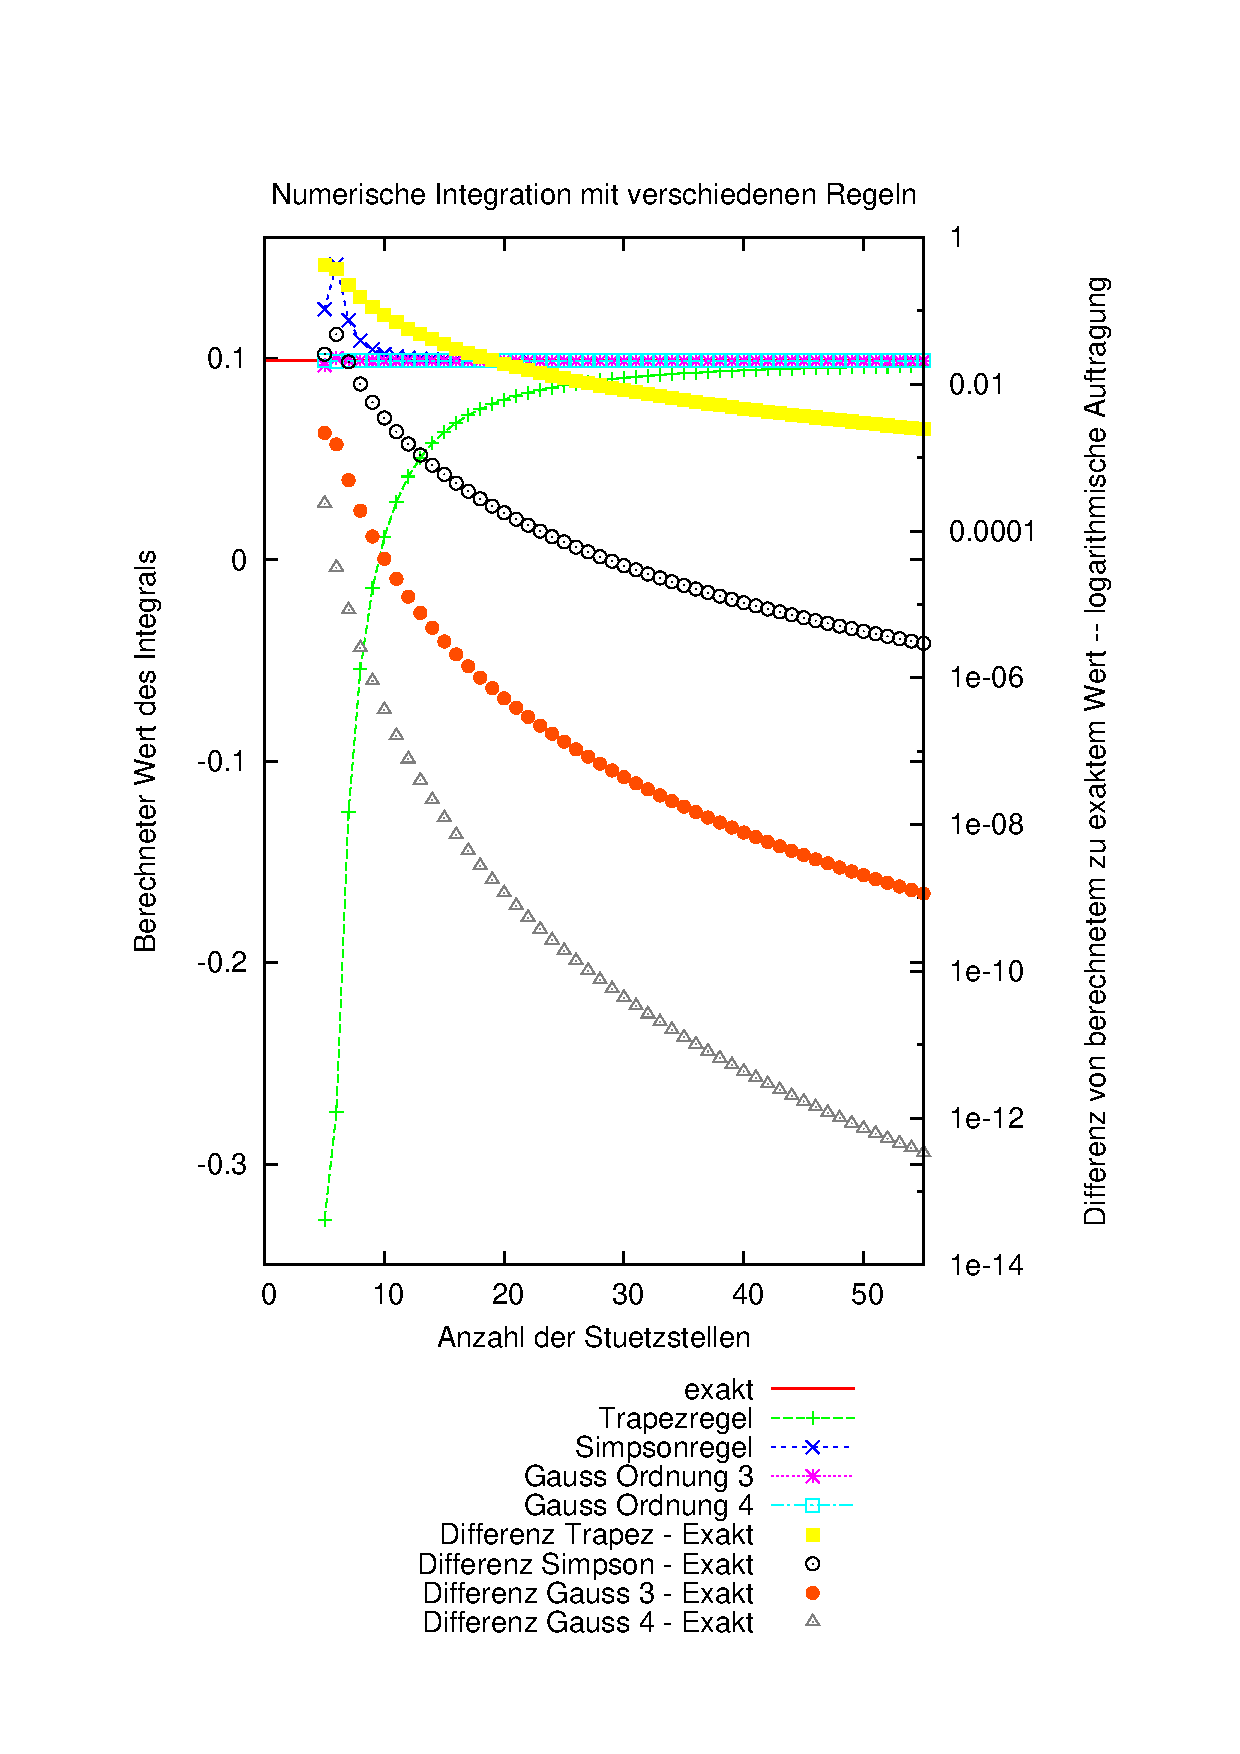
\includegraphics[width=\textwidth]{./bilder/vgl-int}
  \caption{Vergleich verschiedener Integrationsmethoden}
  \label{fig:vgl-integr}
\end{figure}


\section{Adaptive Integration}
\label{sec:adaptive_integration}

Dein einfachste Ansatz ist wie oben schon besprochen, das Intervall
$[a,b]$ zu halbieren, wo $f$ st"arker variiert -- also schwerer zu
integrieren ist.

Man kombiniert dabei zwei Verfahren, mit denen man jeweils das
Teilintervall Integriert und vergleicht anschlie"send die Ergebnisse;
sind diese um mehr als $\varepsilon$ verschieden, wird das betreffende
Intervall wieder halbiert usw.  Elegant kann man dies nat"urlich in
einer Rekursion behandeln.

Die Entscheidung, ob nun geteilt werden soll oder nicht, kann man noch
verfeinern, indem die Abbruchbedingung
\begin{equation*}
  | I_1 - I_2 | < \frac{b_j - a_j}{b-a} \, \varepsilon
\end{equation*}
verwendet -- hier bei ber"ucksichtigt man, dass die Teilintervalle
k"urzer sind und setzt den Integrationsfehler ins Verh"altnis mit der
Intervalll"ange. Ebenfalls kann man einen Relativen Fehler $\delta$
einf"uhren und die Abbruchbedingung
\begin{equation*}
  | I_1 - I_2 | < \delta \, I_S \text{ oder } \frac{I_1}{I_2} < \delta
\end{equation*}
formulieren, wobei $I_S$ ein grober Sch"atzwert f"ur das Integral ist.














\chapter{Einschrittverfahren f"ur Anfangswertprobleme}
\label{cha:einschr_fur_anfangsw}


Ganz allgemein behandeln wir Differenzialgleichungen der Form
\begin{equation}
  \label{eq:16}
  \dot{ \vec y }(t) = \vec f( t, \vec y(t) ) \text{ mit } \vec y(a) =
  y(0) \text{ und } t \in [a,b] \;,
\end{equation}
mit Funktionen $\vec y \in \mathbb R^N$. Um die Schreibarbeit zu
erleichtern werden wir aber in Kurzform schreiben
\begin{equation}
  \label{eq:18}
  y' = f( t, y) \text{ und } y(a) = y_0 \;.
\end{equation}




\begin{Wichtig}
  [Existenz und Eindeutigkeit]
Ist $f$ \emph{Lipschitz-stetig}, also
\begin{equation}
  \label{eq:19}
\exists L ~ \forall t\in [a,b] ~ \forall u,v \in \mathbb R^N ~: ~  \|
f(t, u ) - f(t, v ) \| \leq L \cdot \| u - v \| \;,
\end{equation}
dann existiert genau eine L"osung.
\end{Wichtig}


\paragraph{Auseinanderdriften}
\label{sec:auseinanderdriften}


L"ost man die DGL f"ur identsiches $f$ aber zwei verschiedene
Anfangswerte $y(a) = y_0$ und $\tilde y(a) = \tilde y_0$, dann driften die
beiden L"osungen h"ochstens exponentiell auseinander:
\begin{equation}
  \label{eq:20}
  \| y(t) - \tilde y(t) \| \leq \E^{L \, (t-a)} \, \| y_0 - \tilde
  y_0\| \;.
\end{equation}

\paragraph{Differenzierbarkeit der L"osungen}
\label{sec:differenzierbarkeit_der_losungen}

Au"serdem kann man folgern, dass wenn $f$ $p$-mal partiell
differenzierbar ist, dass $y$ dann $(p+1)$-mal partiell
differenzierbar ist.


\abs
\paragraph{Herleitungen}
\label{sec:herleitungen}
Die hier beschriebenen Herleitungen sind immer nur eine M"oglichkeit;
oft kann man auch durch (a) Raten oder (b) Taylorentwicklung
(auch kombiniert mit (a)) auf die Resultate kommen: Viele Wege f"uhren
nach Rom...




\section{Definition Einschrittverfahren, Verfahrensfehler}
\label{sec:definition_einschrittverfahren}


Allgemein verwenden wir ein diskretes Rechenverfahren; also anstatt
f"ur die L"osung der DGL \eqref{eq:18} ein Funktion $y(t)$ zu
erhalten, bekommen wir Datenpunkte $u_l := u(t_l)$ wobei $u$ die
numerisch gen"aherte L"osung zu $y$ ist und die $\{ t_l \}_l$ ein
diskretes \emph{Gitter}
\begin{equation}
  \label{eq:21}
  \Delta := \{ a = t_0 < t_1 < t_2 < \dots < t_{n-1} < t_n = b \}
\end{equation}
bilden mit den \emph{Schrittweiten}
\begin{equation}
  \label{eq:22}
  h_l = t_{l+1} - t_l
\end{equation}
zwischen den einzelnen Zeitschritten. Im Allgemeinen werden diese
$h_l$ konstant gew"ahlt.


\begin{Def}
  [Einschrittverfahren]
Der N"ahrungswert $u_{l+1}$ f"ur $y$ bei $t = t_{l+1}$ berechnet sich
lediglich aus $t_l$, $u_l$ und der Schrittweite $h_l$ -- h"angt also
explizit nur von dem vorhergehenden Schritt ab.
\end{Def}

Man definiert hierf"ur die \emph{Verfahrensfunktion} $\varphi$ sodass
\begin{equation}
  \label{eq:23}
  u_{l+1} = u_l + h_l \cdot \varphi( t_l , u_l , h_l ) \text{ mit }
  u_0 = y_0 \;.
\end{equation}



\abs
Um die \emph{G"ute} eines Verfahrens bemessen zu k"onnen, f"uhren wir
die \emph{Konvergenzordnung} ein:
\begin{Def}
  [Konvergenzordnung $p \geq 1$]
Gilt f"ur den globalen Verfahrensfehler die Absch"atzung
\begin{equation}
  \label{eq:24}
  \underbrace{\max_l \| u_l - y(t_l) \|}_\text{Glob. Verfahrensfehler}
  \leq C \cdot \left( \max_l h_l \right)^p \;,
\end{equation}
so ordnet man dem Verfahnre die Konvergenzordnung $p$ zu.
\end{Def}
Die Konvergenzordnung entspricht also der Ordnung des Restterms, wenn
man das Taylorpolynom von N"aherung $u$ und Funktion $y$ voneinander
abzieht.

Es gibt nun ein wichtiges Resultat, um die Konvergenzordnung angeben
zu k"onnen; dazu ben"otigen wir:
\begin{Def}
  [Lokaler Verfahrensfehler $\eta(t, h)$]
Der Lokale Verfahrensfehler gibt die Abweichung an, die dem Verfahren
an einer Stelle inh"arent sind:
\begin{equation}
  \label{eq:25}
  \eta(t,h) :=  \underbrace{ y(t) + h \, \varphi( t, y(t) , h)
  }_{\approx y(t+h) } - y(t+h) \;.
\end{equation}
\end{Def}
Man berechnet also die Abweichung, zwischen einer von exakten Werten
$y(t)$ ausgehenden Approximation  mit der Verfahrensfunktion $\varphi$
und dem tats"achlich exakten Wert $y(t+h)$; $\eta$ ist gewisserma"sen
ein Restglied:
\begin{equation*}
  y_{l+1} = y_l + h_l \varphi(t_l, y_l, h_l) - \eta_l \;.
\end{equation*}

Diese Definition dient eigentlich nur f"ur die Definition der
Wichtigen
\begin{Def}
  [(Konsistenz)Ordnung $p \geq 1$]
Gilt die Absch"atzung
\begin{equation}
  \label{eq:65}
  \| \eta( t , h ) \| \leq C \, h^{p+1}
\end{equation}
dann spricht man dem Verfahren die Konsistenzordnung $p$ zu.
\end{Def}

Es gilt jetzt der Wichtige Zusammenhang
\begin{Wichtig}
  Erf"ullt $\varphi$ die Lipschitzbedingung (~\eqref{eq:19} mit der
  Konstanten $L_\varphi$) und hat die \emph{Konsistenz}ordnung $p$ so
  hat das Verfahren die \emph{Konvergenz}ordnung $p$ und der globale
  Fehler ist
  \begin{equation}
    \label{eq:69}
    \max_l \| u_l - y(t_l) \| \leq \frac{C}{L_\varphi} \, \left (
      \E^{L\varphi(b-a)}-1 \right ) \cdot \left ( \max_l h_l \right )^p \;.
  \end{equation}
\end{Wichtig}






\subsection{Einfache Verfahren}
\label{sec:einfache_verfahren}

\subsubsection{Konsistenzordnung $p = 1$: Euler}
\label{sec:konsistenzordnung_p_=_1:_euler}

Das einfachste und anschaulichste -- leider offensichtlich auch
schlechteste -- Verfahren um Anfangswerte zu l"osen besteht darin,
sich an jedem Punkt im Phasenraum um die Strecke $h$ in Richtung der
Ableitung zu bewegen:
\begin{equation}
  \label{eq:euler}
  u_{l+1} = u_l = h_l \, f( t_l , u_l ) \text{ damit } \varphi(t_l,
  u_l) = f(t_l, u_l) \;.
\end{equation}



\subsubsection{Konsistenzordnung $p=2$: Mod. Euler, Heun}
\label{sec:kons_p=2:_mod._euler_heun}

Hier beginnt man mit dem Ansatz
\begin{equation}
  \label{eq:71}
  \varphi(t,u,h) = a_1 f(t,u) + a_2f(t+b_1 h, u+h_2 h f(t,u) )
\end{equation}
und versucht, die Konstanten $a_i$ und $b_i$ optimal zu w"ahlen. Dazu
taylort man $\varphi$ und $y$ in $h$ und vergleicht\footnote{Beachte
  $h \, O(h^2) = O(h^3)$}
\begin{align*}
  \varphi(t+h,y,h) =& &(a_1 + a_2) f(t,y) + h\left ( \frac{\partial
      f}{\partial t} b_1 a_2 + \frac{\partial f}{\partial y} a_2 b_2
  \right ) + O(h^2) \;,\\
  y(t+h) =& y(t) + h \left[ \right . & f(t,y) + \frac{h}{2} \left ( \frac{\partial
      f}{\partial t} + \frac{\partial f}{\partial y}f \right )  +
  O(h^2) \left . \right] \;.
\end{align*}
Hier ergibt sich
\begin{equation*}
  a_1+a_2 = 1 \text{ , } b_1 a_2 = \frac{1}{2} \text{ und } a_2 b_2 =
  \frac{1}{2} \;;
\end{equation*}
das l"asst einen gewissen Spielraum in der Bestimmung der
Koeffizienten.

Man erh"alt f"ur $a_1 = 0, a_2 = 1 \text{ und } b_1=b_2=\frac{1}{2}$
das \emph{Modifizierte Euler-Verfahren}
\begin{equation}
  \label{eq:modeuler}
  \varphi(t,u,h) = f( t+\frac{h}{2} , u+\frac{h}{2} f(t,u) )
\end{equation}
und f"ur $a_1=a_2 = \frac{1}{2} \text{ und } b_1 = b_2 = 1$ das
\emph{Verfahren von Heun}:
\begin{equation}
  \label{eq:73}
  \varphi(t,u,h) = \frac{1}{2} \left (  f(t,u) + f(t+h, u+h f(t,u)
  \right ) \;.
\end{equation}



\subsubsection{Konsistenzordnung $p=3$: Niedriges Runge Kutta}
\label{sec:kons_p=3:_niedr_runge_kutta}




\subsubsection{Konsistenzordnung $p=4$: Klassisches Runge Kutta}
\label{sec:kons_p=4:_klass_runge_kutta}

Es ergibt sich (o.B.)
\begin{equation}
  \label{eq:klrungekutta}
  \varphi(t,u,h) = \frac{1}{6}\left (  k_1 + 2k_2 + 2k_3 + k_4 \right )
\end{equation}
mit
\begin{align*}
  k_1 &=& f(t,u) \\
  k_2 &=& f(t+\frac{h}{2},u+\frac{h}{2} k_1) \\
  k_3 &=& f(t+\frac{h}{2},u+\frac{h}{2} k_2) \\
  k_4 &=& f(t+h,u+h k_3)  \;.
\end{align*}



\subsubsection{Bemerkung zu Runge-Kutta}
\label{sec:bemerkung_zu_runge_kutta}

Die RUnge-Kutta-Verfahren sind weit verbreitet, deswegen auch in
vielen Standardbibliotheken implementiert. Sie haben eine hohe
Genauigkeit (vgl. Abb. \ref{fig:schrittw-euler}) und die Funktion $f$
muss nicht differenzierbar sein -- die M"oglichen Probleme auf die man
das Verfahren anwenden kann sind dementsprechend gro"s. 

Ein bedeutender Nachteil ist jedoch, dass die Funktion $f$ sehr
h"aufig aufgerufen werden muss -- im Falle $p=4$ bspw. f"unf mal, was
sehr aufw"andig wird.

In Listing
\ref{rungekuttamehrdim}
ist eine Implementierung des Verfahrens angegeben: Der harmonische
Oszillator. Hier wurde auch die Energie mitausgegeben, damit man sich
ein Bild machen kann, wie exakt die Verfahren sind. Der Output ist
geplottet in Abb. \ref{fig:rungekuttamehrdim-output}.


\lstinputlisting[label=rungekuttamehrdim,caption=Simulation
Harmonischer Oszillator mit Euler und
Runge-Kutta,language=c++]{./code/einschrmehrdimA01.cpp}

\begin{figure}
  \centering
  \includegraphics[width=\textwidth]{bilder/einschrmehrdimA01-1}
  \caption{Ouptut von Listing \ref{rungekuttamehrdim}.}
  \label{fig:rungekuttamehrdim-output}
\end{figure}





\section{Extrapolation}
\label{sec:extrapolation-1}

Wie auch bei Integralen oder Ableitungen
(vgl. Kap. \ref{sec:extrapolation}) kann man die Genauigkeit mittels
Extrapolation steigern: Ein Wert $u_{l+1}$ wird mit mehreren
Schrittweiten $h_i$ berechnet 
\begin{equation*}
  u_h := u_{l+1}\text{, berechnet mit } h_l = h 
\end{equation*}
und die Werte daf"ur interpoliert -- also die Punktwolke $(h_i
u_{h_i})$. Anschlie"send wird in der Interpolation $h\to 0$
ausgef"uhrt und dieser Wert verwendet.

\abs
F"ur ein Einzelschrittverfahren der Konsistenzordnung $p\geq 1$ kann
man den durch die endliche Gr"o"se von $h$ verursachten fehler
absch"atzen via
\begin{equation*}
  u_h(t) - y(t) = c_p(t) h^p + c_{p+1}h^{p+1} + ... +
  c_{p+r-1}h^{p+r-1} + O(h^{p+r}) \;.
\end{equation*}
Bildet man nun eine Endliche Folge $h_o > h_1 > ... > h_m$ mit $0 \leq
m \leq r$ und approximiert die Punkt $(h_i , u_{h_i})$ mit einem
Polynom 
\begin{equation*}
  P_{0,...,m}(h) = d_0 + d_{p+1}h^{p+1} + ... + d_{p+m-1}h^{p+r-1} \;,
\end{equation*}
dann l"asst sich das Verfahren um die Ordnung $m$ verbessern:
\begin{equation*}
  y(t) = P_{0,...,m}(0) + O(h^{p+m}) \;.
\end{equation*}




\section{Schrittweitensteuerung}
\label{sec:schrittweitensteuerung}

Der Schritt $(t_l, u_l) \to (t_{l+1}, u_{l+1})$ wird mit einem
Zwischeschritt $(t_l, u_l)\to (t_{l+\frac{1}{2}}, u_{l+\frac{1}{2}})
\to (t_{l+1}, u_{l+1})$ gemacht:
\begin{equation}
  \label{eq:75}
  w = u_l + \frac{h_l}{2} \varphi( t_l, u_l , \frac{h_l}{2} \text{ und
  } u_{l+1} = w + \frac{h_l}{2} \varphi(t_{l} + \frac{h_l}{2} , w ,
  \frac{h_l}{2} ) \;.
\end{equation}

Es soll nun die Schrittweite $h_l$ so gew"ahlt werden, dass f"ur einen
fest gew"ahlten absoluten Fehler $\varepsilon > 0$
\begin{equation}
  \label{eq:76}
  \| u_{l+1} - z(t_l + h_l) \| \approx \varepsilon \;,
\end{equation}
wobei $z$ eine  L"osung f"ur $z' = f(t,z)$ mit $z(t_l) = u_l$ ist.

Dieses "`$\approx$"' macht deshalb Sinn, weil bei gro"sen Fehlern
genauer approximiert werden soll, das $h$ f"ur kleine Fehler aber
ruhig gr"o"ser werden darf, weil man sonst Rundungsfehler bekommen
kann. 

Analog kann man auch als Abbruchbedingungen
\begin{equation*}
   \varepsilon_1 \leq \| u_{l+1} - z(t_l + h_l) \| \leq \varepsilon_2
\end{equation*}
w"ahlen.

Das $z$ muss logischerweise auch mit einem anderen Verfahren bestimmt
werden -- oder man sch"atzt den gesamten Fehler $\| \cdot \|$ ab.
Sei $\tilde
u$ der mit  \eqref{eq:75} bestimmte Wert $u_{l+1}$, dann kann man setzen
\begin{equation}
  \label{eq:77}
  z_h = \tilde u - \frac{u_l + h\varphi(t_l, u_l, h) - \tilde
    u}{2^p-1} = z(t_l+h) + O(h^{p+2}) \;,
\end{equation}
wobei man f"ur den Fehler in \eqref{eq:76} die Absch"atzung
\begin{equation}
  \label{eq:70}
  \delta(h) = \| \tilde u = z_h \| = \frac{\| u_l + h \varphi(t_l,
    u_l, h) - \tilde u \|}{2^{p}-1}
\end{equation}
erh"alt -- was offensichtlich proportional zum Fehler zwischen dem
Verfahren mit und dem ohne Zwischenschritt ist; besagter Faktor ergibt
sich aus diversen Rest-Absch"atzungen.

Erf"ullt dieses $\delta(h) \approx \varepsilon$, so kann man das $h$
verwenden. Wenn nicht, so muss man $h \mapsto h' < h$.

Dieses $h'$ w"ahlt man (f"ur $h \ll \varepsilon^{1/(p+2)}$) am besten
via
\begin{equation}
  \label{eq:72}
  h' = \left ( \frac{\varepsilon}{\delta(h)} \right )^{1/(p+1)} \cdot
  h \;,
\end{equation}
was sich aus weiteren Restterm-Absch"atzungen ergibt. Daraus folgt
auch, dass ein g"unstiger Startwert
\begin{equation}
  \label{eq:74}
  h_0 = \varepsilon^q ~ \text{ mit } 1 < q < \frac{1}{2+p}
\end{equation}
ist.

\abs
Der Algorithmus ist also insgesamt:
\begin{enumerate}
\item W"ahle $h = h_0$ nach \eqref{eq:74}. \label{item:1algoschritt}
\item Berechne aus $u_l$: $u_{l+1}$ und $\tilde u$
\item Sch"atze den Fehler ab mit \eqref{eq:70}
\item Ist die Bedingung \eqref{eq:76} erf"ullt, so w"ahle $u(t_{l+1})
  = \tilde u$; wenn \emph{nicht}, so verfeinere $h$ mittels
  \eqref{eq:72} und beginne wieder bei \ref{item:1algoschritt}.
\end{enumerate}

\paragraph{Energieerhaltung}
\label{sec:energieerhaltung-1}

Eine elegante Methode in Systemen mit erhaltener Energie ist auch,
anstatt der Forderung \eqref{eq:76} zu verlangen, dass $\Delta E <
\varepsilon$ wobei $\Delta E$ die Abweichung der aktuell berechneten
Energie zur tats"achlichen Energie (die man ja aus den
Anfangsbedingungen berechnen kann) ist.

\begin{figure}
  \centering
  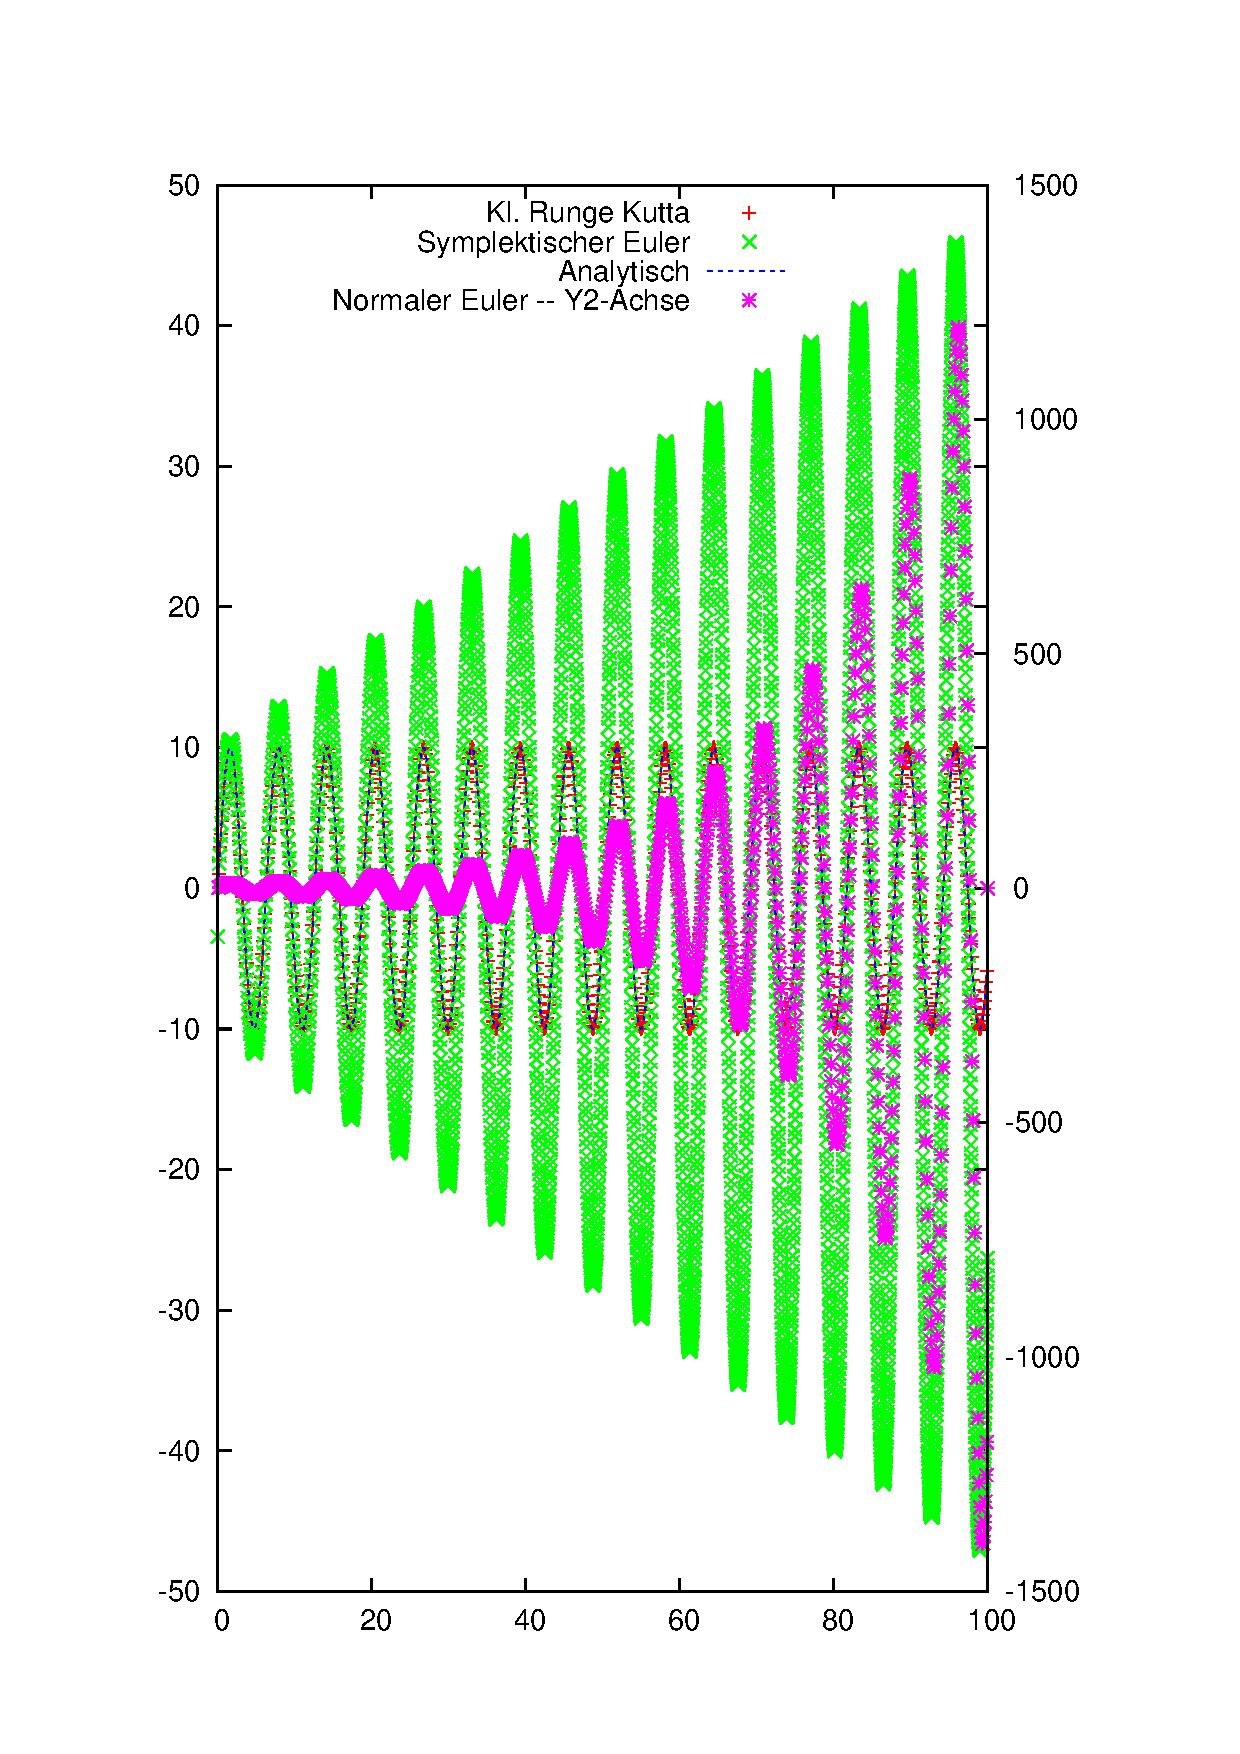
\includegraphics[width=\textwidth]{bilder/vorteil-symplekt-1}
  \caption{Vergleich zwischen normalem Euler, Euler mit Schrittweitensteuerung durch Energierhaltung und Runge Kutta f"ur den Harmonischen Oszillator}
  \label{fig:schrittw-euler}
\end{figure}

In Abb. 
\ref{fig:schrittw-euler}
ist dargestellt, wie sich die Integration damit verbessert: Hier sieht
man auf der Y2-Achse wie starkt das normale Eulerverfahren
auseinanderdriftet. F"ur das "`symplektische"' Verfahren wurde die
Schrittweite jedes mal halbiert, wenn die Differenz zwischen aktueller
und vorhergehender Energie gr"o"ser als $0.5$ war (die Energie f"ur
die Anfangsbedingungen betrug $50$).

Im Gegensatz dazu sieht man aber auch, wie gut das
Runte-Kutta-Verfahren funktioniert -- jedoch muss man bedenken, dass
der Aufwand hier auch \emph{wesentlich} h"oher ist.

Vergleiche zu dieser Idee auch Kap. \ref{sec:symplektische_integration}.






\section{Symplektische Integration}
\label{sec:symplektische_integration}

Die Symplektische Integration ist ein Verfahren, bei dem physikalische
Gegebenheiten eingesetzt werden, um -- physikalische --
Differenzialgleichungen exakter integrieren zu k"onnen. Grundlage dazu
bildet der Hamiltonformalismus, wobei f"ur uns n"otig ist, dass sich
der Hamiltonian $H$ schreiben l"asst via
\begin{equation}
  \label{eq:78}
  H(p,q) = T(p) + V(q) \;.
\end{equation}
Mit den Hamilton-Jacobi-DGL
\begin{equation}
\label{eq:79}
  \dot p = - \frac{\partial H}{\partial q} = - \frac{\partial
    V}{\partial q} \text{ und } \dot q = \frac{\partial H}{\partial p}
  = \frac{\partial T}{\partial p}
\end{equation}
f"ur den Spezialfall \eqref{eq:78} kann man Verfahren herleiten, bei
denen die Gesamtenergie $T+V$ besser erhalten
bleibt\footnote{Pr"aziser: es bleibt das Phasenraumvolumen $\diff p
  \wedge \diff v$ erhalten}, als bei vergleichbaren Verfahren
"ahnlicher Ordnung. 

Dazu betrachtet man Bewegungen als Vektor $\vec z = (q , p)^T$; dann
ist die Bewegungsdgl
\begin{equation}
  \label{eq:80}
  \dot{\vec z} =
  \begin{pmatrix}
    \frac{\diff }{\diff t} & 0 \\
    0 & \frac{\diff }{\diff t}
  \end{pmatrix} \cdot \vec z
=: D_H \vec z = (D_T + D_V)\vec z \;,
\end{equation}
wobei die letzte Gleichung sich ergibt, weil man diese Gleichung mit
den Poissonklammern auch als\footnote{Vlg auch Von-Neumann-Gl. oder
  allgemein Hamilton-Formalismus}
\begin{equation*}
  \dot{\vec z} = \{ \vec z , H \} = \{ \vec z , T \} + \{\vec z , V \}
\end{equation*}
schreiben kann. Eine DGL der Form \eqref{eq:80} l"ost man durch den
Exponentialmatrixansatz:
\begin{equation}
  \label{eq:81}
  \vec z(t) = \exp( t D_H ) \,\vec z(0) = \exp( t D_T + t D_V ) \,\vec z(0) \;.
\end{equation}
Diese Exponentialfunktion kann man nun umschreiben in ein Produkt
$$
\exp[t (D_T + D_V)] = \prod_{i=1}^k \exp(c_i t D_T)\exp(d_i t
D_V) + O(t^{n+1}) \;,
$$
mit gewissen Koeffizienten $c_i$ und $d_i$. $k \in \mathbb N$ hei"st
\emph{Ordnung} des Verfahrens. F"ur die einzelnen "`kleinen"'
Exponentialmatrizen gilt nun 
$$
\exp(c_i t D_T) : \begin{pmatrix}
q\\ p
\end{pmatrix}
\mapsto
\begin{pmatrix}
q'\\ p'
\end{pmatrix}
=
\begin{pmatrix}
 q + t c_i \frac{\partial T}{\partial p}(p)\\
 p
\end{pmatrix}
$$
und
$$
\exp(d_i t D_V) : \begin{pmatrix}
q\\ p
\end{pmatrix}
\mapsto
\begin{pmatrix}
q'\\ p'
\end{pmatrix}
=
\begin{pmatrix}
 q \\
 p - t d_i \frac{\partial V}{\partial q}(q)\\
\end{pmatrix} \;.
$$


\subsection{Euler-Chromer-Verfahren}
\label{sec:euler_chromer_verfahren}

F"ur $k=1$ und die Zahlen $c_1 = d_1 = 1$ erh"alt man so\footnote{das
  Produkt der Exponentialmatrizen ist als Komposition von rechts nach
  links zu verstehen} f"ur $t = \Delta t = h$ f"ur den Zeitschritt $t \to t+\Delta t$:
\begin{align}
  \label{eq:83}
  v_{n+1} &= v_n + h \, g( t_n , y_n ) \\
  y_{n+1} &= y_{n} + h \, v_{n+1}  \;,
\end{align}
wobei $g$  von der DGL $\ddot y = g(t, y)$
kommt.


\subsection{Verlet-Methode}
\label{sec:verlet_methode}

F"ur $k=2$ und mit $c_1 = c_2 = \frac{1}{2}$, $d_1 = 1$ und $d_2 = 0$
erh"alt man
\begin{equation}
  \label{eq:82}
  y_{l+1} = 2 y_l - y_{l-1} + h^2 \, g(t,y_l)
\end{equation}
wobei $g$ wieder die Zweite Ableitung bezeichnet: $\ddot y = g(t,y)$.

Dies ist eine Methode der Ordnung $4$ -- aber eigentlich ist es kein
klassisches Einschrittverfahren, weil auf der rechten Seite auch
$y_{l-1}$ auftaucht.







\subsubsection{Energieerhaltung}
\label{sec:energieerhaltung}

Diese Methode eignet sich nat"urlich gut, wenn man eine Funktion
integrieren will, bei der die Energie erhalten bleibt -- beim
angegebenen Hamiltonian \eqref{eq:78} ist das der Fall. Sobald jedoch
Reibungskr"afte etc. (Dissipative Elemente in $H$) auftreten, wird das
Verfahren nicht mehr so gut sein...




\section{Chaos}
\label{sec:chaos}




\section{Molekulardynamik}
\label{sec:molekulardynamik}

Hier betrachtet man $N$ Teilchen -- jedoch mit sehr gro"sen $N$ -- die
miteinander wechselwirken, bspw. Gase, Fl"ussigkeiten, Membrane,
Sch"uttg"uter, Molek"ule, Atome, \dots. Hier kommt es im Allgemeinen
nicht unbedingt zu genau auf die einzelnen Bahnen der Teilchen an,
sondern auf das Verhalten der Gesamtheit -- dementsprechend ist man
meits nur an Gr"o"sen interessiert, die die Gesamtheit der Teilchen
konstituieren, bspw. Temperatur, Druck, Spannung, \dots.

In der Praxis sind hierbei noch $N \sim 10^8$ Teilchen
praktikabel. W"ahlt man bspw. f"ur Atome $\Delta t \sim
10^{-12}\operatorname{s}$, dann kann man $\sim 10^6$ Zeitschritte weit
berechnen, also $t \sim 1\operatorname{\mu s}$.

\paragraph{Optimierungen}
\label{sec:optimierungen}

Wenn jedes Teilchen mit jedem anderen in
Wechselwrikung tritt, und man m"ochte jede einzelne der
Wechselwrikungen berechnen, dann hat man (unter Ausnutzung von Actio =
Reactio) $\frac{N(N-1)} 2 = O(N^2)$ Wechselwirkungen zu berechnen. Im
Gegensatz zu bspw. Himmelsmechanik, wo man eine langreichweitige
Wechselwirkung (Gravitation) betrachtet, kann man im Allgemeinen die
Kraft eines Teilchens auf die Kraft reduzieren, die es auf seine (mehr
oder weniger direkten) Nachbarn aus"ubt -- i.A. also nur Teilchen,
f"ur die der Abstand $< R$ ist. In der Praxis verwendet man f"ur dieses $R$:
\begin{equation*}
  R \sim 2.5 \, \lambda \;,
\end{equation*}
wobei $\lambda$ der \emph{Mittlere Teilchenabstand} ist. Dies ist
jedoch sehr stark abh"angig von der Weitreichweitigkeit der Wechselwirkung.

Um dies Effektiv
durchzuf"uhren gibt es mehrere Verfahren:
\begin{description}
\item[Nachbartafeln] auch \emph{Verlet-Tafeln} genannt: F"ur jedes
  Teilchen wird eine Liste der Nachbarn mit $r < R'$ gef"uhrt. Es
  m"ussen dann nur diese untersucht werden, ob $r < R$ ist.

  Der Aufwand hierf"ur -- die Listen zu aktualisieren -- ist jedoch
  auch $O(N^2)$; der Nutzen ist nicht gro"s. Es sei denn, dass man die
  Listen nicht nach jedem Zeitschritt aktualisiert, sondern erst nach mehreren!
\item[Linked Lists] Auch \emph{Zell-Listen genannt}: Der Raum wird in
  Zellen (ein Gitter) mit Kantenl"ante $R$ aufgeteilt und nur Teilchen in den benachbarten
  Feldern m"ussen beachtet werden. Die Aktualisierung dieser Liste ist
  nur $O(N)$ aufw"andig, weil man nur "uber alle Teilchen Iterieren
  muss um diese einer Zelle zuzuweisen.
\item[Kombination] Der Nachteil der Linked Lists ist nat"urlich, dass
  die Wechselwirkung im Allgemeinen Symmetrisch sein wird -- also
  einen Ball mit Radius $R$ um jedes Teilchen aufspannt, wohingegen
  die Zellen Eckig sind: Der Abstand zweier Teilchen in benachbarten
  Zellen kann so -- wenn sie genau auf der Diagonalen sitzen -- auch
  $\sqrt 2 R$ betragen. Das kann man entsch"arfen, indem man f"ur die
  Teilchen einer Zelle wieder jeweise Nachbartafeln f"uhrt.
\end{description}



\chapter{Mehrschrittverfahren f"ur Anfangswertprobleme}
\label{cha:mehrschr_fur_anfangsw}

todo...







\chapter{Stochastik und Statistik}
\label{cha:stochastik_und_statistik}


\section{Einf"uhrung Statistik}
\label{sec:einfuhrung_statistik}


\subsection{Definitionen}
\label{sec:definitionen}


\begin{Def}
  [Mittelwert $\mittel \cdot$]
Von einer Messreihe $x_i$ mit $i  \in \{ 1, ..., N \}$ definiert man
\begin{equation}
  \label{eq:84}
  \mittel x := \frac{1}{N} \, \sum_{i = 1}^N x_i \;.
\end{equation}
\end{Def}
Logischerweise ist hier die Reihenfolge der Messwerte nicht
entscheidend.

In der Statistik spricht man vom $k$-ten \emph{Moment}, wenn man
$\mittel{ x^k }$ meint und vom $k$-ten \emph{zentralen Moment},
wenn man $\mittel{ (x-\langle s  \rangle)^k}$ meint. Diese
zentralen Momente gleichen den Momenten aus der Physik: Interpretiert
man die $x_i$ als die Abst"ande von Massepunkten der Masse $1$, so
beschreibt $\mittel x$ den \emph{Schwerpunkt}, das zweite
"`mechanische Moment"' -- also das Tr"agheits\emph{moment} --
entspricht dem zweiten zentralen Moment:

\begin{Def}
  [Varianz $\sigma$] Die Varianz zum Quadrat ist das mittlere
  Abweichungsquadrat vom Mittelwert:
  \begin{equation}
    \label{eq:85}
    \sigma^2 := \mittel{ (x-\langle x  \rangle )^2 }
= \mittel{ x^2  } - \mittel{ x  }^2
  \end{equation}
\end{Def}
Die Gleichung erh"alt man direkt wenn man die Definition von $\mittel
\cdot$ stur anwendet und die binomische Formel beachtet.

Nun definiert man noch weiter den 
\begin{Def}
  [Statistischer Fehler $\Delta$]
  \begin{equation}
    \label{eq:86}
    \Delta := \frac{\sigma}{\sqrt{ N - 1}}
  \end{equation}
\end{Def}
Dieser hat den Vorteil, dass man eine Messreihe aufteilen kann in
kleinere Messreihen: Berechnet man hier jeweils die Mittelwerte 
und bildet aus diesen Mittelwerte der Untermessreihen eine weitere
Messreihe, so kann man f"ur beide Datens"atze -- den urspr"unglichen
und den bereits "`vorberechneten"' -- den statistischen Fehler
bestimmen und diese werden gleich sein. Bei der Varianz wird diese
jedoch nicht so sein; hier wird durch die Aufteilung noch ein Faktor
$1/m$ (wenn $m$ die Anzahl der Untermessreihen ist) auftauchen.


\subsection{Lineare Regression}
\label{sec:lineare_regression}

Seien $N$ Datenpunkte $(x_i, y_i)$ gegeben ($i \in \{ 1, ..., N
\}$). Durch diese wollen wir eine Gerade $y = m x + b$ so legen, dass
die Punkte m"oglichst gut in der $\ell^2_N$ Norm
\begin{equation}
  \label{eq:87}
  \| y_i - y(x_i) \| = \frac{1}{N} \sum_{i = 1}^N ( y_i - (mx_i +b)
  )^2 =
\mittel{  ( y - (mx +b))^2 }
=: S
\end{equation}
approximiert werden kann. Nun soll $S$ extremal werden, also sollen
die Abl. nach $m$ und $b$ verschwinden:
\begin{equation*}
  \frac{\partial S}{\partial m} = \mittel{  -2x ( y - (mx +b)) }
= -2 \left (\mittel{ xy } - m \mittel{ x^2 } - b \mittel x \right ) = 0
\end{equation*}
und
\begin{equation*}
  \frac{\partial S}{\partial b} = \mittel{ -2 (y-(mx+b)) } = -2 \left(
    \mittel y - m \mittel x + b \right ) = 0 \;.
\end{equation*}
Das lineare Gleichungsstystem aus diesen beiden Gleichungen kann man
nun l"osen und erh"alt
\begin{equation}
  \label{eq:88}
  m = \frac{\mittel{ xy} + \mittel{x} \mittel y}{\mittel{ x^2 } +
    \mittel{x}^2} \text{ und } b = m \mittel x - \mittel y \;.
\end{equation}
Damit braucht man nur eine Funktion f"ur $\mittel \cdot$ zu
implementieren und hat schon ein Programm mit dem man lineare
Regression durchf"uhren kann.

\abs
M"ochte man \emph{noch} exotischere Funktionen als $mx + b$ anfitte,
muss man versuchen, diese durch Skalierung der Axen auf eine Gerade zu
bekommen; bspw kann man aus der Exonentialfunktion $f(x) = A\, \exp(b
\, x)$ durch Logarighmieren $g(x) = \ln f(x) = \ln A + b x$ machen und
hat -- voil\'a -- eine Funktion mit der unser Programm etwas anfangen
kann. 

Das Problem ist nat"urlich, dass jetzt nicht mehr die Norm
\eqref{eq:87} verwendet wird sondern eine transformierte Version
davon...




\section{Zufallsgeneratoren}
\label{sec:zufallsgeneratoren}



\begin{Def}
  [Zufallszahlen]
Eine Folge $(a_k)_k$ von Zahlen in unkorellierter Reihenfolge -- also bei der
man nicht von einer (oder mehreren benachbarten) Zahl(en) auf die
Folgezahl schlie"sen kann. Die Wahrscheinlichkeit, welchen Wert $a_k$
annimmt, soll f"ur alle m"oglichen Zahlen gleich sein.
\end{Def}

Wir m"ochten im Folgenden Kapitel mit Zufallszahlen arbeiten um
stochastische Modelle zu simulieren. Das Problem ist nur, dass ein
Ergebnis in der Physik -- bzw der Wissenschaft
allgemein\footnote{Beachte: Chemie $\not \subseteq$ Wissenschaften} --
reproduzierbar sein soll.

Verwendet man also f"ur eine Simulation \emph{echte} Zufallszahlen,
wie man sie beispielsweise aus Rauschen in der Hardware (unter Linux kann
man dazu \texttt{/dev/random} verwenden), einem
Geigerz"ahler oder "ahnlichem erhalten kann, dann wird die Simulatin
stets andere Ergebnisse liefern.

Stattdessen verwendet man bestimmte Generatoren, die --
reproduzierbare -- \emph{Pseudo-Zufallszahlen} bereitstellen.



\subsection{Kongruentieller Zufallsgenerator RNG ("`IBM"')}
\label{sec:kongr_zufallsg_rng_ibm}

Aus dem $i$-ten Element wird das $(i+1)$-te Berechnet via
\begin{equation}
  \label{eq:89}
  x_{i+1} = (c \, x_i ) \mod p
\end{equation}
mit einer \emph{Primzahl} $p$. $p$ muss prim sein, weil sich sonst
$\mod p = 0$ ergeben kann; dann w"aren alle weiteren Zahlen $0$.

Die erste Zahl $x_0$ bezeichnet man als \emph{Seed} (Keim): Mit diesem
Seed und $c$ und $p$ ist die Folge reproduzierbar.

Weil die Folge jedoch nur vom Vorg"anger abh"angt, wird sie
unweigerlich periodisch: Sobald eine Zahl nochmal vorkommt, m"ussen
auch alle Zahlen hinter dieser Zahl sich wiederholen. Diese
"`Periodendauer"' ist maximal $p$ weil $p\mod p = 0$ und $(p+k)\mod p
= k \mod p$.

F"ur gute Generatoren muss also $p$ gro"s genug sein, dass die Periode
nur einmal durchlaufen wird. Gute Ergebnisse erh"alt man, wenn $p$
eine \emph{Mersenne-Primzahl} $M_n = 2^n-1$ ist -- hier ist $n$ auch
prim!. Weiter folgt aus der Zahlentheorie dass
\begin{equation*}
  c^p \mod p = 1 \text{ und } \not \exists q < p \text{ mit } c^q \mod
  p = 1 \;.
\end{equation*}

IBM benutzte in den ersten 32-bit Komputern
\begin{equation*}
  p = 2^{31} -1 \text{ und } c = 2^{16}-3 \;.
\end{equation*}
Dieser generator l"asst sich in Assembler schnell und elegant
implementieren; er kann $2^{31}-1 \sim 10^{9.6}$ verschiedene
Zufallszahlen erzeugen, bevor er periodisch wird.

Diese Generatoren sind heute \emph{out of date}.




\subsection{Lagged-Fibonacci-Sequenz}
\label{sec:lagged_fibonacci_sequenz}

Hier h"angt $x_{i+1}$ von zwei Vorg"angern ab:
\begin{equation}
  \label{eq:90}
  x_{i+1} = (x_{i-a} + x_{i-b}) \mod \beta
\end{equation}
liefert Zufallszahlen in Basis $\beta$ -- also f"ur $\beta=2$ bin"ar, f"ur
$\beta=64$ W"orter, etc.

Sei oBdA $a>b$, dann braucht man als "`Startwerte"' mindestens $a$
Zufallszahlen -- die man dann wieder mit einem Verfahren aus
Kap. \ref{sec:kongr_zufallsg_rng_ibm} bereitstellen muss.

Mit viel Zahlentheorie kommt man f"ur $a$ und $b$ auf die Bedingung,
dass es sich um ein \emph{Zierlertrinom}
\begin{equation*}
  T_{ab} = 1+z^a + z^b
\end{equation*}
handeln muss mit bin"aren $z$; $T_{ab}$ darf sich nicht in
Unterpolynome faktorisieren lassen.

Hier verwendet man Zufallszahlen bis zu $100\, 000$ und erh"alt so bei
einer Periodizit"at von $2^a-1 = 10^{\log 2 \cdot 100\,000}-1 \sim
10^{30\,100}$ wesentlich mehr Zahlen als mit dem multiplikativen
Verfahren.



\section{Testen von Zufallszahlen}
\label{sec:testen_von_zufallszahlen}

Mit folgenden Verfahren kann man die \emph{G"ute} von Zufallszahlen
bestimmen:
\begin{description}
\item[Graphisch] Zwei (drei) aufeinanderfolgende Zufallszahlen werden
  als zweidimensionale (dreidimensionale) Koordinaten eines
  kartesischen Koordinatensystems gedeutet und darsgestellt. F"ur gute
  Zufallszahlen (also zuf"allige) ergibt sich ein homogenes Bild, f"ur
  schlechte ein Muster.
\item[Mittelwert] F"ur Zufallszahlen aus $[a,b]$ sollte $\mittel x =
  \frac{b-a}{2}$ sein.
\item[Gau"s Glocke] Ein Histogramm der Daten soll eine Gau"s-Glocke ergeben.
\item[Fourieranalyse] Das Spektrum der Zufallszahlen als (st"uckweise
  stetige bzw Treppen-) Funktion gedeutet soll glatt sein -- bei
  Spitzen hat man Resonanzen, also sich wiederholende Muster.
\item[Korellation] Es sollte
  \begin{equation}
    \label{eq:91}
    \mittel{ x(a) \cdot x(b) } = \delta_{a,b}
  \end{equation}
gelten, wobei $x(\xi)$ die um $\xi$ verschobenen Zufallszahlen $x_{i +
  \xi}$ sind. Es solls ich also nur wenn die beiden Folgen wirklich
identisch sind eine Korellation zwischen den beiden ergeben.
\end{description}








\chapter{Popylationsdynamik}
\label{cha:popylationsdynamik}


\section{Eine Spezies}
\label{sec:eine_spezies}


\subsection{Einfachste Modelle}
\label{sec:einfachste_modelle}


\paragraph{Exponentielles Wachstum}
\label{sec:exponentielles_wachstum}

Geht man von dem einfachen Modell aus, dass eine Spezies eine gewisse
Geburtenrate $b$ und eine Mortalit"atsrate $m$ hat, so ergibt sich aus
einer Population von $P_n$ Wesen nach einem Zeitschritt
\begin{equation*}
  P_{n+1} = b \, P_n - m \, P_n = \alpha \, P_n \;, \text{ und damit }
  P_n = \alpha^n P_0 \;.
\end{equation*}

In Form von Differenzialgleichungen bekommt man die rate $\alpha$ in
die "Anderung der Population:
\begin{equation*}
  \dot y = \tilde\alpha \, y \text{ und damit } y(t) = \E^{\tilde\alpha t} y(0) \;.
\end{equation*}


\paragraph{Logistisches Wachstum}
\label{sec:logistisches_wachstum}

Ber"ucksichtigt man dar"uber hinaus noch die Kapazit"at $k$ eines gewissen
Lebensraumes, so d"ampft diese im einfachsten Modell das Wachstum
$\alpha$ dahingehend, dass die Vermehrung nur noch mit $\alpha' =
(\alpha - k \, P_n$ stattfindet: Je gr"o"ser die Population bereits
ist, desto weniger stark kann sich die Population vermehren. In
Diskreter Form f"uhrt dies auf
\begin{equation*}
  P_{n+1} = (\alpha - k P_n) P_n
\end{equation*}
und in differenzieller auf
\begin{equation*}
  \dot y = (\tilde\alpha - \tilde k y) y \;.
\end{equation*}

Diese Form kann man l"osen und findet die drei Funktionen:
\begin{equation*}
  y_1 = \frac{\tilde \alpha / \tilde k}{1+(\frac{\tilde\alpha / \tilde
    k}{y_0} - 1 ) \E^{-\tilde\alpha t}} , y_2 = 0 ,
  y_3 = k
\end{equation*}

\paragraph{Unterschied diskret--differenziell}
\label{sec:unterschied_diskret_differenziell}

Bei der Formulierung mit DGLs kann man das "`Arsenal"' der Analysis
auffahren und die Gleichungen l"osen (versuchen) -- in diskreter Form
fehlen diese Hilfsmittel. F"ur gro"se Populationen ist es auch nicht
mehr relevant, ob man mit einer Funktion bspw. $149.23$ oder $149$
Wesen ausrechnet -- der Unterschied kann getrost Vernachl"assigt
werden.

Wieter ist wichtig, dass bei den differenziellen Modellen eine
Zeitskala gegeben ist -- die man auch weiter verfeinern kann.

Nachteile sind jedoch, dass 
\begin{itemize}
\item kleine "Anderungen haben gro"sen Einfluss
\item Erzwingen einer gew"unschten Population -- sp"ater eines
  bestimmten Verh"altnisses -- ist schwierig
\end{itemize}



\subsubsection{Rauschen}
\label{sec:rauschen}

Um die Stabilit"at einer L"osung zu testen, adiert man ein
\emph{Rauschen}, bspw.
\begin{equation*}
  \xi = A \cos(t)
\end{equation*}
mit $A \ll y_0$ ($A$ soll gegen $y$ klein sein) und betrachtet dann in
der DGL $y_\xi = y + \xi$. Wenn das Ergebnis dadurch nur ein wenig
"`wackelt"' hat man einen stabile L"osung gefunden und eine instabile,
wenn die L"osung sich sofort stark ver"andert.







\section{Zwei und mehr Spezies}
\label{sec:zwei_und_mehr_spezies}

Hier betrachtet man meist zwei Konkurrenten; bspw. R"auber und
Beutetiere.

Diese Modelle sind jedoch nach wie vor Simpel, weil sie keinerlei
Fluktuationen aufweisen und nicht r"aumlich aufl"osen -- also die
Formeln sind so, als w"urden sich alle Tiere an einem Ort aufhalten.

\subsection{Einfaches Modell: Volterra-Gleichung}
\label{sec:einf_modell:_volt_gleich}

Die Kapazit"aten seien unbegrenzt; die Beutetiere sterben nur, wenn
sie gefressen werden und die R"auber sterben nur, wenn sie nicht genug
Beute bekommen -- also verhungern. Die Geburtenrate ist proportional
zur Population. 

Bezeichne Beute mit $y_1$ und R"auber mit $y_2$; $m$ ist die
Mortalit"atsrate, $b$ die Geburtenrate:
\begin{align}
  \label{eq:volt-beute}
  \dot y_1 &= (b_1 - r_{21} y_2 ) y_1 \;,\\
  \label{eq:volt-raeuber}
  \dot y_2 &= (-m_2 + R_{12} y_1 ) y_2 \;.
\end{align}





\subsection{Lotka-Gleichung}
\label{sec:lotka_gleichung}

Das System wird entwas verfeinert: Die Zahl der B"autetiere ist jetzt
durch eine Kapazit"at begrenzt; zu \eqref{eq:volt-raeuber} kommt jetzt
\begin{equation}
  \label{eq:lotka-beute}
  \dot y_1 = (b - r_{21}y_2 - \frac{1}{k} y_1 ) y_1 \;.
\end{equation}

Der neue Term $y_1/k$ wirkt wie eine Reibung auf das System; es ist
m"oglichk, dass es zu Gleichgewichten kommt und das Aussterben von
Arten ist m"oglich.




\section{Diskrete Modelle}
\label{sec:diskrete_modelle}

Den in \ref{sec:zwei_und_mehr_spezies} angesprochenen M"angeln
versucht man jetzt zu begegnen: Der Lebensraum der Wesen wird in ein
Gitter zerlegt und pro Gitterfeld werden Zahl und Spezies
festgehalten.

In dem neuen Modell gibt es jetzt Aktivit"aten; bspw
\begin{description}
\item[Migration] Mit bestimmter Wahrscheinlichkeit bewegt isch ein
  Tier auf einen anderen Platz
\item[Jagd] R"auber machen Beute, wenn die Beutetiere in einer
  gewissen Umgebung sind
\item[Geburt/Tod] Satte R"auber haben mehr Nachkommen, hungrige
  sterben; Tiere sterben durch Alter ...
\end{description}

Beobachtet man ein solches System, so bemerkt man, dass das Verhalten
stark von der Gr"o"se des Lebensraumes abh"angig ist:
\begin{description}
\item[zu klein] Die Beute wird ausgerottet -- und die R"auber damit auch
\item[mittel] Die Best"ande oszillieren
\item[zu gro"s] Populationen sind i.A. konstant, nur kleine Fluktuationen
\end{description}

F"ur diese Modelle ist es offensichtlich n"otig, sich von einer
deterministischen Beschreibung des Systems zu l"osen und zu einer
stochastischen "uberzugehen: Bei den einzelnen Aktionen soll der
\emph{Zufall} eine (gro"se) Rolle spielen. 

Um solche Systeme also zu modellieren, sind gute
Zufallszahlen-Generatoren n"otig -- Vgl
Kap. \ref{sec:zufallsgeneratoren}.




\section{Zellularautomaten}
\label{sec:zellularautomaten}

Bei zellul"aren Automaten hat man einen Raum -- ein \emph{Spielfeld}
-- vorliegen, welches durch ein Gitter in diskrete Positionen
aufgeteilt ist. Jeder Gitterpunkt kann besetzt oder nichtbesetzt sein
und in jedem Zeitschritt entscheide sich, ob ein Gitterpunkt weiterhin
besetzt oder unbesetzt sein wird alleine durch die Anzahl von
besetzten Gitterpunkten in seiner Nachbarschaft. In jedem Zeitschritt
wird also nach und nach f"ur jeden Gitterpunkt eine Dynamik-Regel
angewandt, welche ihre Entscheidungsgrundlage aus der vorhergehenden,
abgeschlossenen Runde nimmt.


\subsection{Beispiel: Regel 90}
\label{sec:regel_90}


Ein Beispiel f"ur einen solchen Automat ist ein $N$-Eck, dessen Ecken
entweder $1$ oder $0$ haben/sein k"onnen. Wenn in der vorhergehenden
Runde genau einer der beiden Nachbarn $1$ hatte, wird in der aktuellen
Runde die Ecke $1$ haben, ansonsten $0$.

Ist $f(i)$ der Wahrheitswert an der $i$-ten Stelle so gilt
\begin{equation*}
  f'(i) = (f(i+1) \wedge \neg f(i-1)) \vee (\neg f(i+1) \wedge  f(i-1))
\end{equation*}
wobei der $'$ bedeuten soll, dass es sich um den n"achsten Zeitschritt handelt.

Bin"ar sieht diese Regel so aus -- hier sind in der Vorg"angerreihe
nebeneinander linker Nachbar, Punkt selbst, rechter Nachbar:

\begin{tabular}{l c c c c c c c c}
  Vorg"anger & 000 & 001 & 010 & 011 & 100 & 101 & 110 & 111 \\
  Nachfolger & 0   & 1   & 0   & 1   & 1   & 0   & 1   & 0
\end{tabular}

Stephen Wolfram f"uhrte hierf"ur ein Klassifikationssystem ein,
demnach wird diese Regel mit
\begin{equation*}
0 \cdot 2^0 + 
1 \cdot 2^1 + 
0 \cdot 2^2 + 
1 \cdot 2^3 + 
1 \cdot 2^4 + 
0 \cdot 2^5 + 
1 \cdot 2^6 + 
0 \cdot 2^7 = 90 
\end{equation*}
bezeichnet.



\subsection{Randwert"ubertrag}
\label{sec:randwertubertrag}

Oft identifiziert man die R"ander einer Simulation miteinander;
d.h. die Teilchen "`ganz links"' haben auch Nachbarn "`ganz
rechts"'. Um dies umzusetzen gibt es zwei Methoden:
\begin{description}
\item[Pointer] Eine Pointerfunktion $P_l(i)$ zeigt stets auf den
  linken Nachbarn vom Feld $i$, $P_r(i)$ auf den Rechten. Diese
  Funktionen m"ussen stets abfragen, ob sie jetzt "uber einen Rand
  gegangen sind oder nicht. Die Problematik wird also in eine einfache
  \texttt{if}-Abfrage ausgelagert.
\item[Schattenfelder] F"uhre Neben den Feldern $1,...,N$ noch $0$ und
  $N+1$ ein. Dynamik-Funktion $f$ kann jetzt einfach ihre
  "`physikalischen"' Nachbarn abfragen. Am Ende jeder Runde m"ussen
  die Schattenfelder aktualisiert werden, also der Wert von Feld $1$
  nach $N+1$ geschrieben werden und der von $N$ nach Feld $0$.
\end{description}



\subsection{Beispiel: Game of Live}
\label{sec:beispiel:_game_of_live}

In einem zweidimensionalen Zellautomaten mit Quadratgitter ist jede
Zelle entweder leer oder besetzt. Ob eine Zelle in der n"achsten Runde
besetzt ist, h"angt von der Anzahl $k$ der Nachbarn ab:
\begin{enumerate}
\item $k > 3$: "Uberbev"olkerung f"urht zu Aussterben: $f' = 0$.
\item $k = 3$: Idealbev"olkerung: $f' = 1$.
\item $k = 2$: Keine Ver"anderung: $f' = f$.
\item $k < 2$: Vereinsamung f"uhrt zu Aussterben: $f' = 0$.
\end{enumerate}




\section{Random Walks}
\label{sec:random_walks}

Um ungerichtete Bewegungen zu simulieren -- bspw. Brown'sche
Bewegungen, Diffussion -- ist es nicht m"oglich/n"otig/sinnvoll f"ur
jedes Teilchen eine exakte Trajektorie zu berechnen vielmehr verfolgt
man einen stochastischen Ansatz: Durch Kollisionen und andere
Wechselwirkungen, die man nicht im Detail zu wissen braucht, kommt es
st"andig zu zuf"alligen Richtungs"anderungen. In
Abb. \ref{fig:vgl-real-rw} ist der Vergleich zwischen einem real
gemessenen und einem simulierten Random Walk abgebildet. 


\begin{figure}
  \centering
    \subfigure{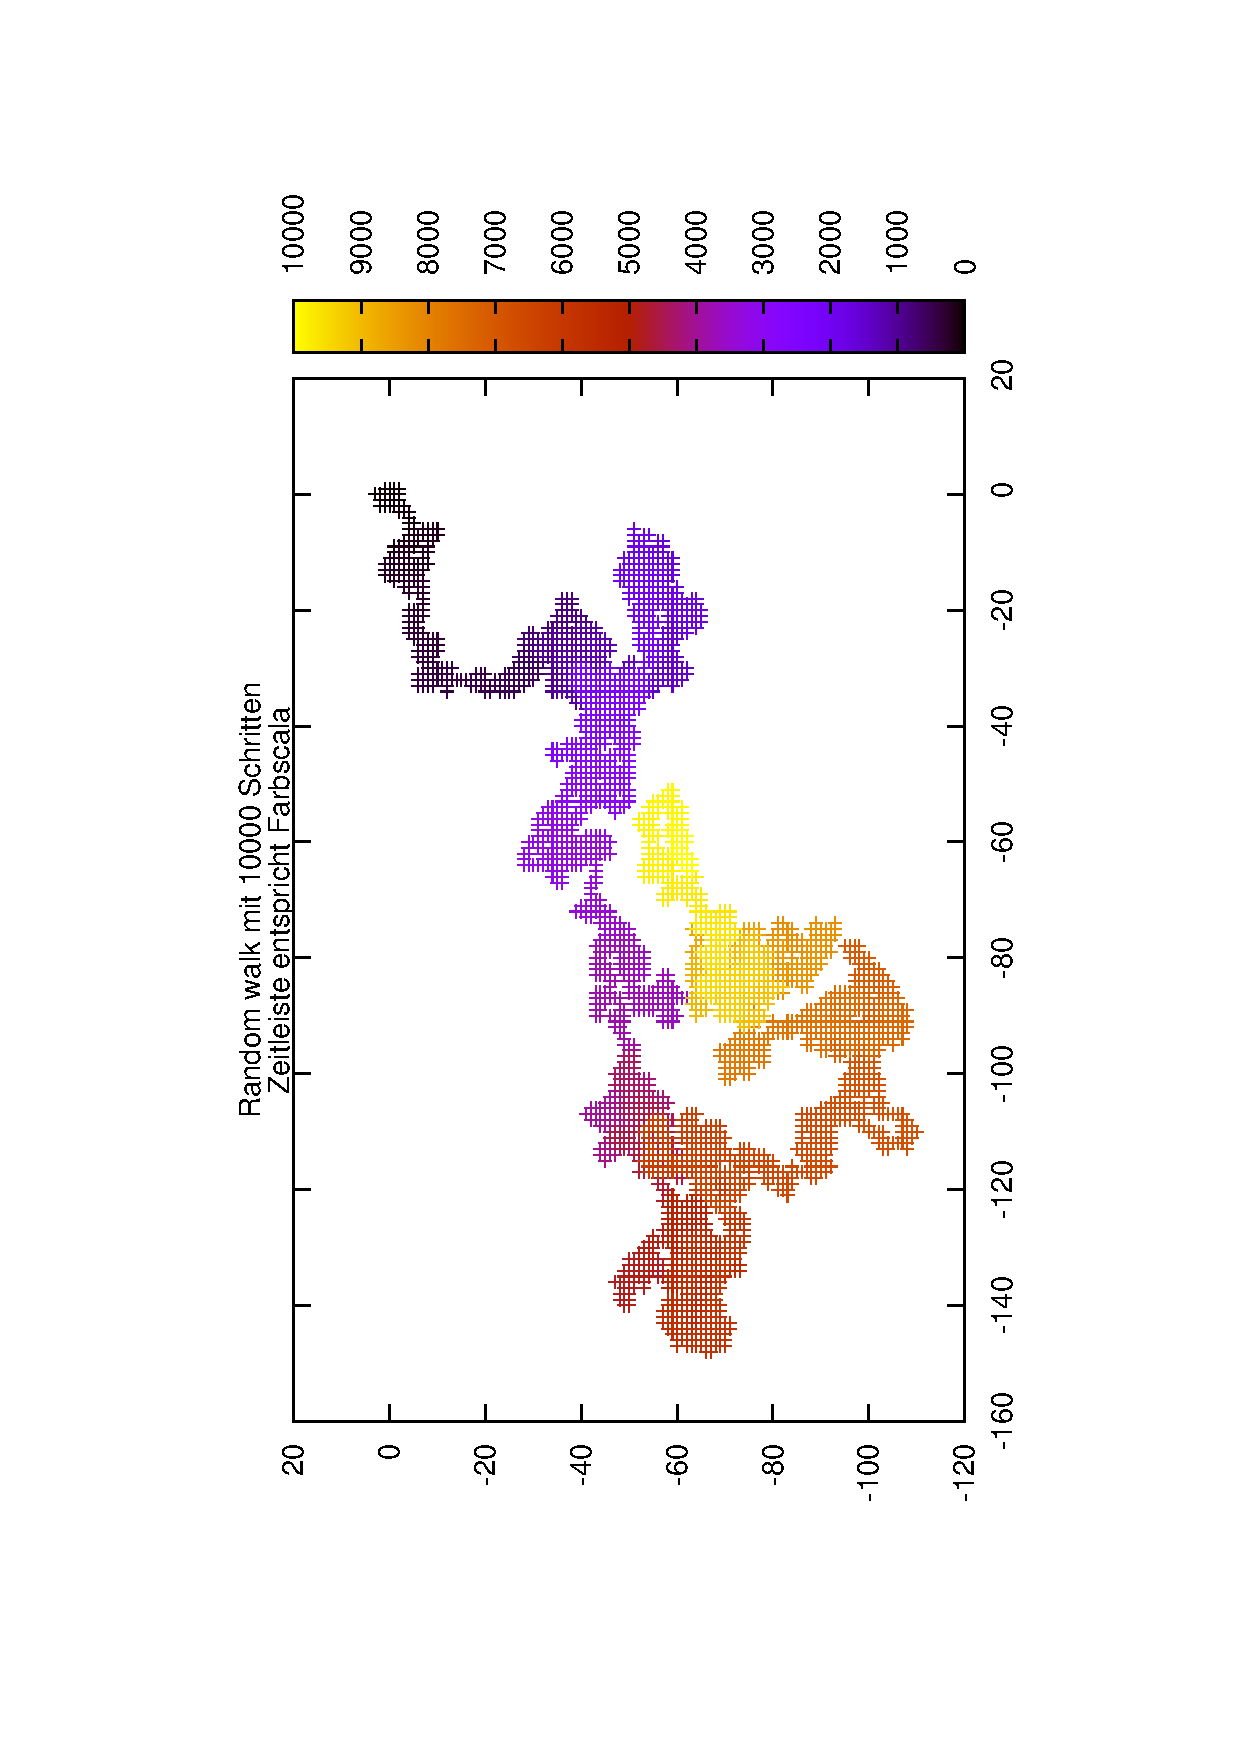
\includegraphics[angle=-90,width=\textwidth]{bilder/rw-10000-2}}
    \subfigure{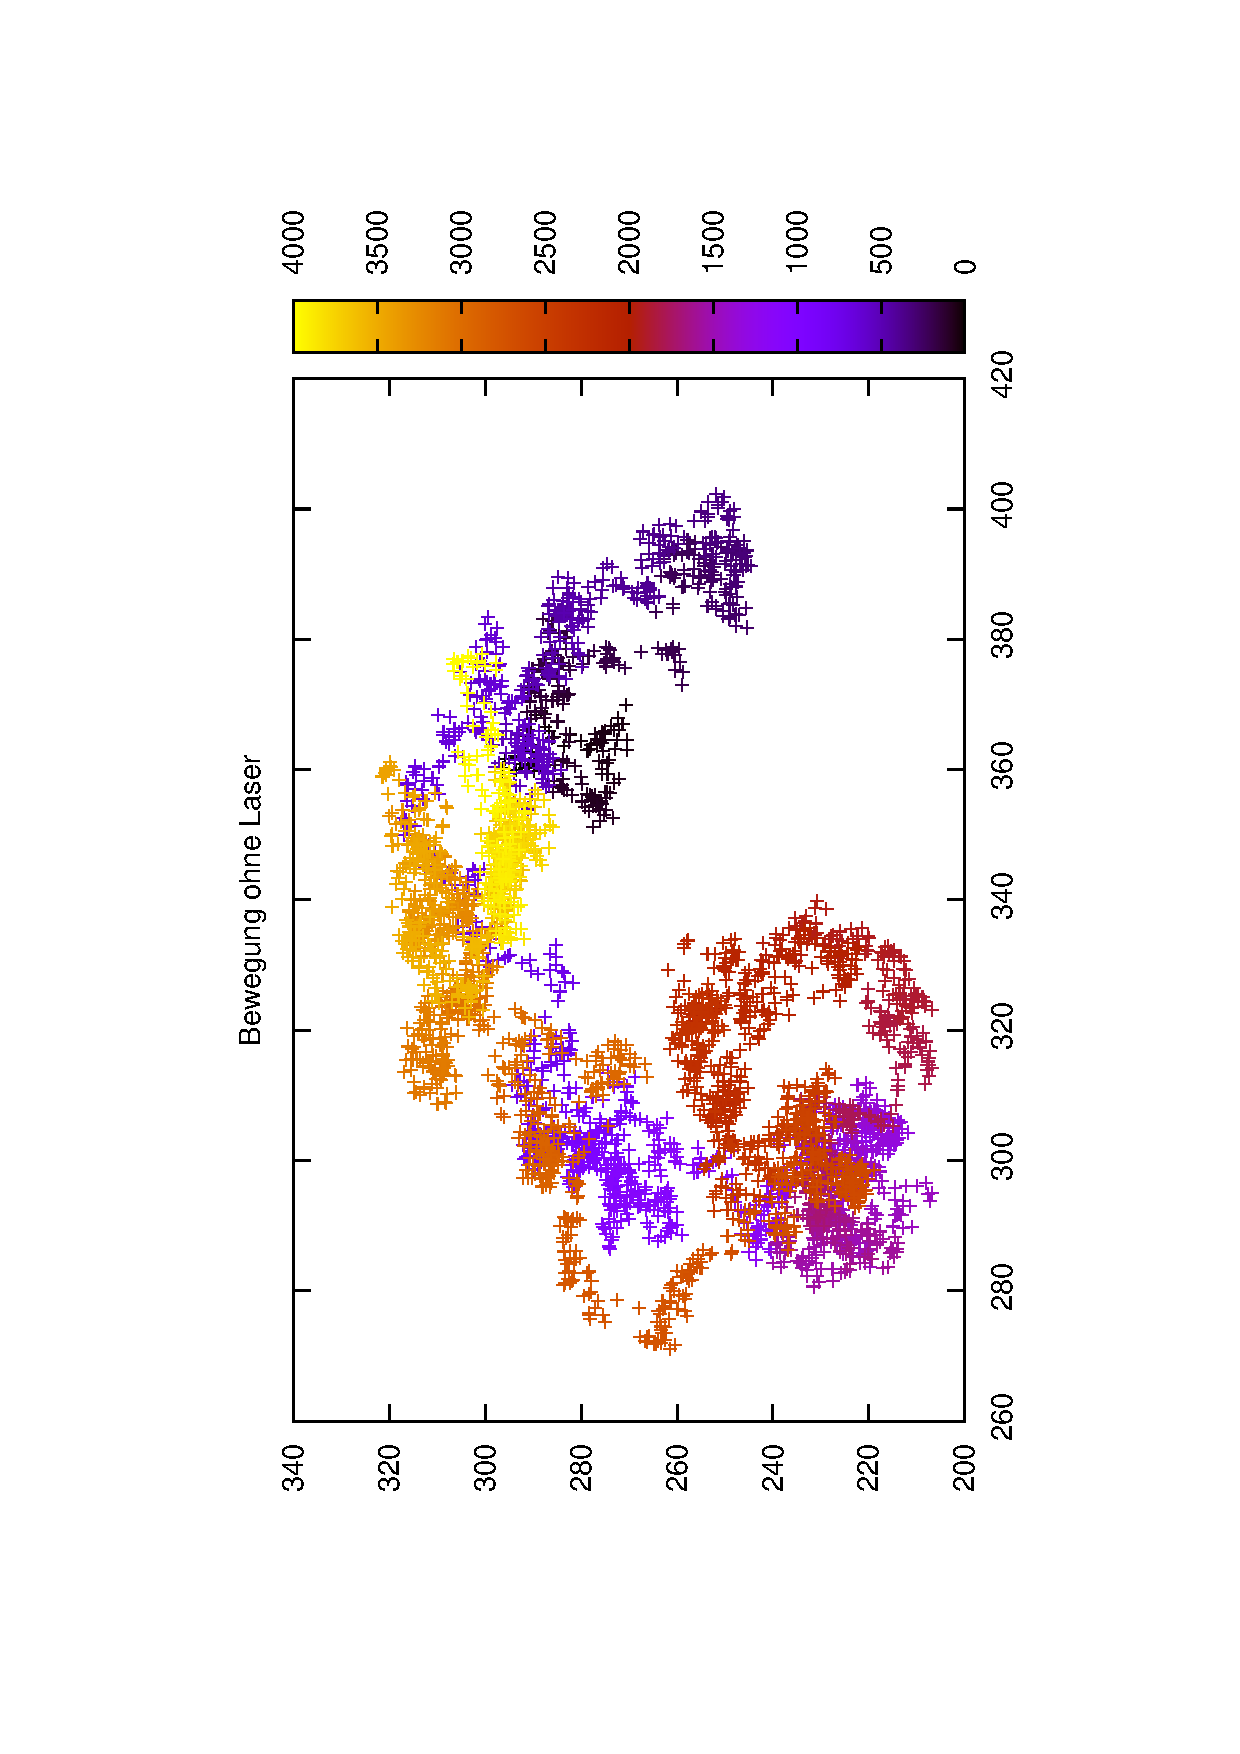
\includegraphics[angle=-90,width=\textwidth]{bilder/rw-real}}
  \caption{Vergleich der Simulierten und einer realen Bewegung
    (thermische Bewegung eines Kolloidteilchen) mit Ranom Walk}
  \label{fig:vgl-real-rw}
\end{figure}


Im einfachsten Modell hat man ein diskretes eindimensionales Gitter
auf dem ein Teilchen mit der gleichen Wahrscheinlichkeit nach rechts
oder links springt. Der diskrete Ort nach $i$ Zeitschritten ist damit
$x_i = \sum_{k = 0}^i \gamma_k$, wobei $\gamma_k \in \{-1,1\}$ die
Richtung des n"achsten Zeitschritts angibt.

$\mittel \cdot$ beschreibt die Mittlung "uber $N$ Zeitschritte. Wir
wollen $\mittel {x^2}$ bestimmen. Dabei ist
\begin{equation*}
  x_t^2 = \left( \sum_{k=0}^t  \gamma_k \right)^2 = \sum_{k.j}\gamma_k\gamma_j
\end{equation*}
und hier kann man nun verwenden, dass f"ur $k \neq j$ ~ $\gamma_k\gamma_j \in \{-1,+1\}$
liegt -- und zwar mit gleicher Wahrscheinlichkeit: Diese Terme knallen
sich in der Summe also \emph{im Mittel} weg und "Ubrig bleiben nur die Terme
$\gamma_k\gamma_k$ und diese sind stets $1$; damit folgt
\begin{equation}
  \label{eq:92}
  \mittel {x^2} = D \, t
\end{equation}
mit der \emph{Diffusionskonstanten} $D$; in unsererm Falle ist $D =
1$. Die Ausbreitung erfolgt damit im Mittel mit 
\begin{equation}
  \label{eq:93}
  \sqrt{ \mittel{ x^2 } } = \sqrt { D t } \propto \sqrt t \;.
\end{equation}

Macht man $N$ Random Walks mit jeweils der Dauer $T$, so erh"alt man
als Ergebnis standardverteilte Endpunkte, wie sie bspw. in
Abb. \ref{fig:distrrandomw500000} zu sehen sind. Hier ist eine
Gau"sglocke angefittet um zu zeigen, wie genau die Positionen dieser
Verteilung folgen.

Dies kann man analytisch herleiten, indem man sich die
Wahrscheinlichkeit $p = p(x,t)$ anschaut, an einem Ort $x$ zur Zeit
$t$ ein Teilchen zu finden:
\begin{equation*}
  \Delta p(x,t+\Delta t) = p(x+\Delta x,t) w_- + p(x-\Delta x,t) w_+ -
  p(x,t)(w_+ + w_-) \;.
\end{equation*}
Die "Anderung der Besetzungswahrscheinlichkeit bei $x$ in einem
Zeitschritt $\Delta t$ h"angt von der Wahrscheinlichkeit ab, dass der
Nachbar $x+\Delta x$ besetzt ist und dort ein Teilchen
"`runter"'springt -- $w_-$ -- und ebenso beim anderen Nachbarn und
au"serdem von der Wahrscheinlichkeit daf"ur, dass das Feld bereits
besetzt ist und ein Teilchen in irgendeine (also eine der beiden
m"oglichen) Richtungen springt. 

Daraus erh"alt man mit $w_- = w_+$ im Grenz"ubergang die DGL\footnote{Vgl W"armeleitgleichung}
\begin{equation*}
  \frac{\partial p}{\partial t} = D \frac{\partial ^2 p}{\partial x^2}
\end{equation*}
indem man $p(x+\Delta x,t) w_-  - p(x,t) w_- \to w_- \frac{\partial
  p(x,t)}{\partial x} \Delta x$ gehen l"asst, analog den zweiten Term
gegen $w_+ \frac{\partial p(x-\Delta x,t}{\partial x}\Delta x$,
hiervon wieder den Differenzenquotienten bildet und schlie"slich $D =
\frac{w \, \Delta x^2}{\Delta t}$ setzt. Eine L"osung dazu ist
\begin{equation*}
  p(x,t) = \frac{1}{\sqrt{2\pi} \sigma} \exp\left(
    \frac{-(x-\mu)^2}{2\sigma^2} \right ) \text{ mit } \sigma = \sqrt{
    2 D t } \;,
\end{equation*}
also eine auseinanderflie"sende Gau"sglocke.




\begin{figure}
  \centering
  \includegraphics[angle=-90,width=0.45\textwidth]{bilder/randoms-500000.histo.eps}
  \caption{Verteilung der X-Koordinate nach 500000 Random Walks;
    Gau"sglocke angefittet}
  \label{fig:distrrandomw500000}
\end{figure}




\section{Weitere Beispiele f"ur stochastische Simulationsmodelle}
\label{sec:weit_beisp_fur_stoch_simul}





\subsection{Perkulation}
\label{sec:perkulation}


Ein "`Spielfeld"' ist in ein diskretes Gitter unterteilt. Die
einzelnen Gitterpunkte ("`Felder"') werden mit einer bestimmten
Besetzungswahrscheinlichkeit $p$ besetzt -- oder eben nicht
--. Anschlie"send z"undet man alle besetzten Felder in einer Randzeile
an und diese wiederum z"unden ihre direkten Nachbarn an. 

Eine \emph{Perkulation} findet per Definiton genau dann statt, wenn
sich das "`Feuer"' bis an den entgegengesetzten Rand durchgearbeitet
hat.

F"ur ein bestimmtes System untersucht man nun die Wahrscheinlichkeit
$p_c$, ab der ($p > p_c$) eine Perkulation wesentlich wahrscheinlicher
wird als die Nicht-Perkulation.

Damit kann man bspw. -- woraus sich die Begrifflichkeit oben herleitet
-- $\star$ ein bewachsenes Waldst"uck simulieren, in dem ein Feuer ausbricht
oder $\star$ Wasser, das durch por"oses Gestein ab einer bestimmten
Por"osit"at durchflie"sen kann oder $\star$ eine Mischung aus
Isolator/Leiter-Pulver, das ab einem bestimmten Anteil Leiter erst
leitet u.v.m. simulieren.

Die \emph{Perkulationsschwelle} $p_c$ h"angt dabei nur von der
Geometrie des Problems ab: F"ur ein Quadratgitter in zwei Dimensionen
gilt $p_c \approx 0.592745$ und f"ur ein Dreiecksgitter in zwei
Dimensionen $p_c = 0.5$.

In Listing \ref{perkulation} ist ein Beispielcode aufgef"uhrt die hier
verwendete Klasse "`Spielfeld"' stellt einfach nur ein Gitter von
Bools zur Verf"ugung, das ausgegeben, einzelne Felder gesetzt und zwei
Spielfelder verglichen werden k"onnen; vgl. \ref{spielfeld}.

\lstinputlisting[label=perkulation,caption=Code f"ur eine Perkulation]{./code/perk.cpp} 


\begin{lstlisting}[caption=Spielfeld.h,label=spielfeld]{Spielfeld.h}
#ifndef SPIELFELD_H
#define SPIELFELD_H

#include<cstdlib>
#include<iostream>

static double zufall()
{
        return double(rand())/RAND_MAX;
}


class Spielfeld {
        private:
                int breite, hoehe;
                bool *felder;
                char ausgabedevice;
        public:
                // constructon
                Spielfeld(int, int, double);
                // getter
                bool operator() (int, int);
                // setter
                void set(int, int, bool);
                // nachtraeglich besetzen
                void zufaellig_besetzen(double);
                // output
                void ausgeben(); // nur ein Spielfeld ausgeben
                void diff_ausgeben(Spielfeld &); // verknuepfung von zwei ausgeben
                
};


Spielfeld::Spielfeld(int breiteP, int hoeheP, double besetzungswahrscheinlichkeit) 
: breite(breiteP), hoehe(hoeheP), felder( new bool[ breiteP*hoeheP ] )
{
       
        for( int i = 0; i < breite; i++ )
                for( int j = 0; j < hoehe; j++ )
                        felder[j*hoehe + i] = ( besetzungswahrscheinlichkeit > zufall() );
}

bool Spielfeld::operator() (int x, int y)
{
        // abfrage ob felder sinnvoll sind
        if( ( 0 <= x) && (x < breite) && ( 0 <= y ) && ( y < hoehe ) )
                return felder[y*hoehe + x];
        // wenn nicht: false ausgeben [felder ausserhalb des spielfelds sind nicht besetzt...]
        else return false;
}

void Spielfeld::set(int x, int y, bool foo)
{
        // abfrage ob felder sinnvoll sind
        if( ( 0 <= x) && (x < breite) && ( 0 <= y ) && ( y < hoehe ) )
                felder[y*hoehe + x] = foo;
        // wenn nicht: stirb
        else std::exit(1);
}

void Spielfeld::ausgeben()
{
                        
         for( int j = 0; j < hoehe; j++ )
         {
                  for( int i = 0; i < breite; i++ )
                  {
                            if( felder[j*hoehe+i] ) std::cout << "#" ;
                            else std::cout << " ";
                  }
                  std::cout << "\n";
         }
}

void Spielfeld::diff_ausgeben(Spielfeld &foo)
{



      for( int j = 0; j < hoehe; j++ )
      {                          
                for( int i = 0; i < breite; i++ )
                {
                         if( felder[j*hoehe+i] && foo(i,j) ) std::cout << "@" ;
                         else
                         {
                                if( felder[j*hoehe+i] && ( ! foo(i,j) ) ) std::cout << "#" ;
                                else std::cout << " ";
                         }
                 }
                 std::cout << "\n";
       }
}

#endif
\end{lstlisting}



In Abb. \ref{fig:schwelle-perk} sieht man, wie die
Perkulationswahrscheinlichkeit mit gr"o"serer
Besetzungswahrscheinlichkeit zunimmt und f"ur $p \approx 0.5923$
gerade im Sprung nach oben begriffen ist -- das deckt sich recht gut
mit den theoretischen Werten oben.

\begin{figure}
  \centering
  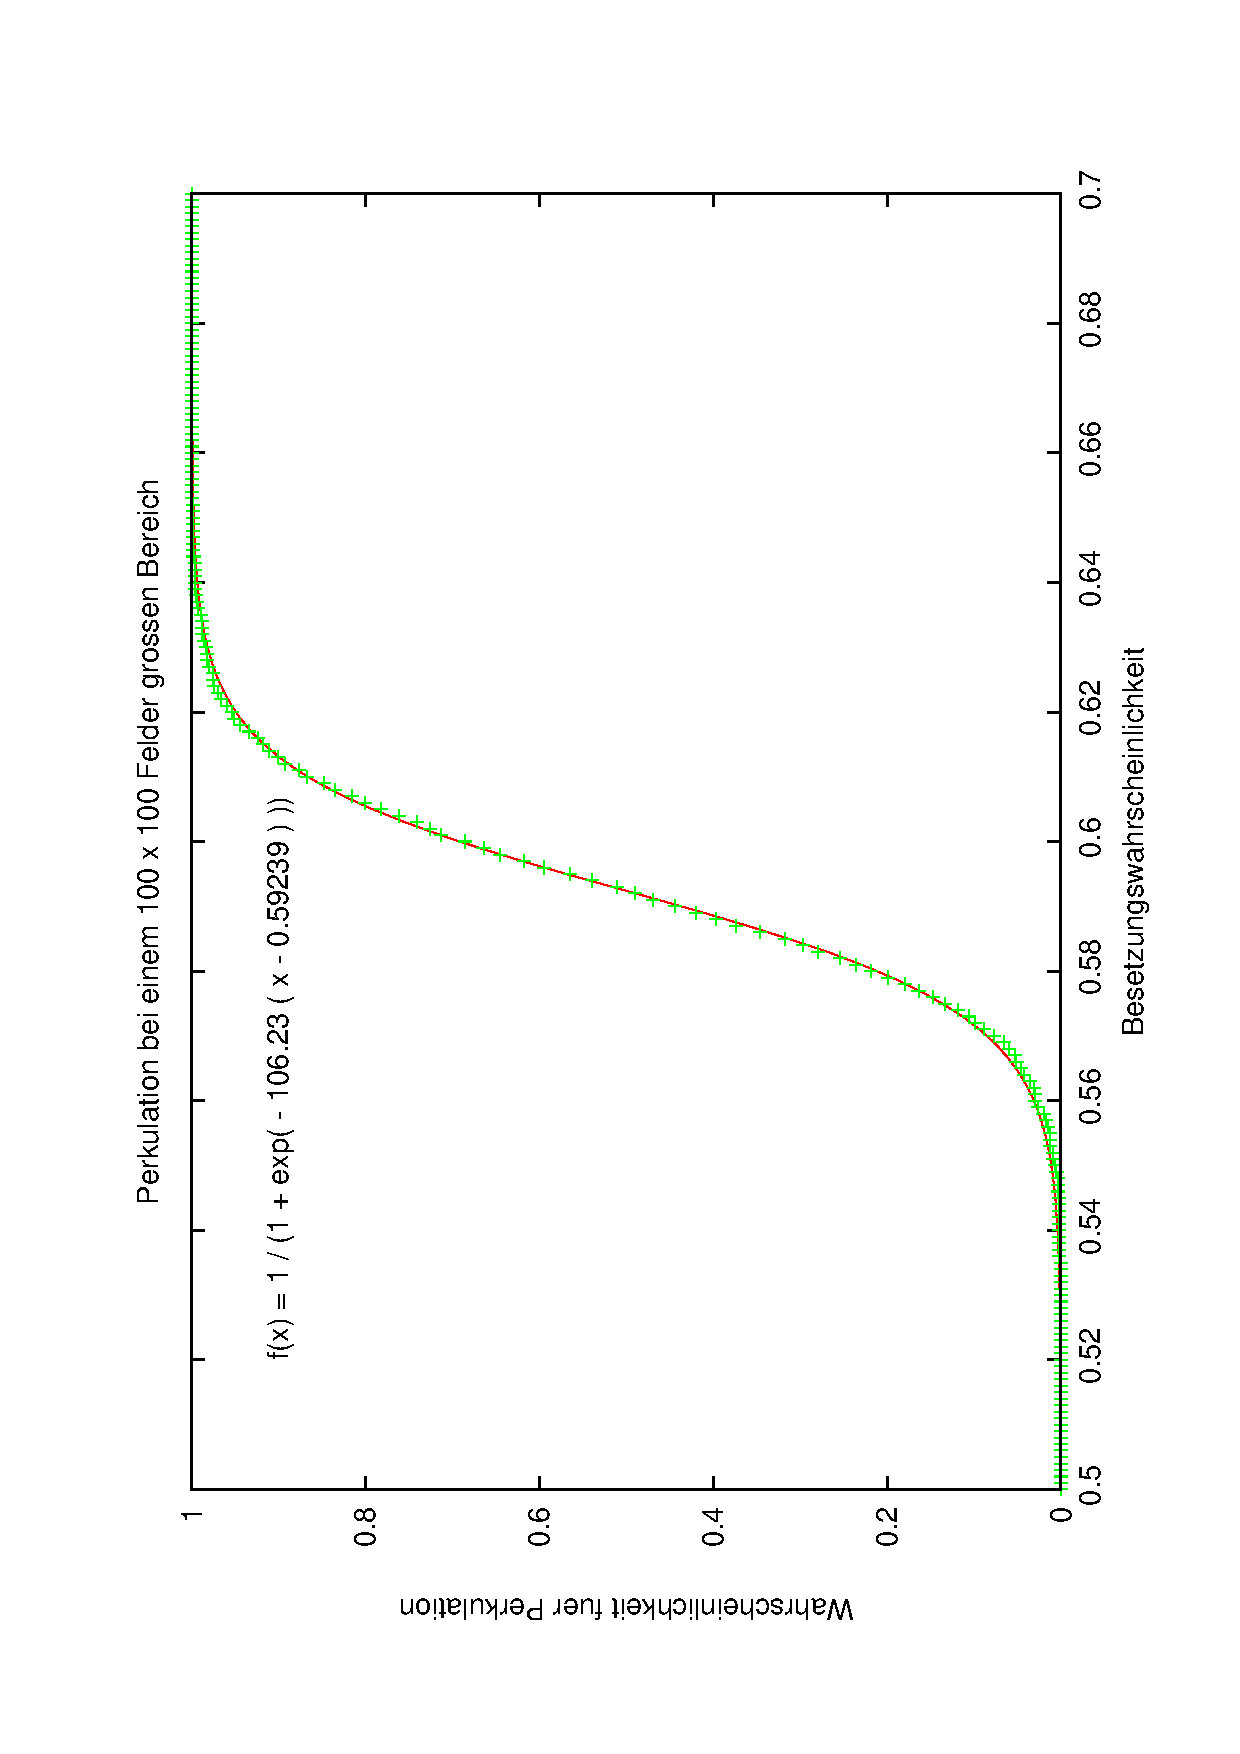
\includegraphics[angle=-90,width=0.45\textwidth]{bilder/schwelle-2}
  \caption{Perkulationswahrscheinlichkeit in Abh"angigkeit der Besetzungswahrscheinlichkeit}
  \label{fig:schwelle-perk}
\end{figure}





\subsection{Eden-Modell}
\label{sec:eden_modell}


Hiermit simuliert man pspw die Ausbreitung von Tumoren (daf"ur wurde
die Simulation entwickelt!) etc. Der Ablauf
ist wie folgt: Eine einzelne infizierte Zelle wird in die Mitte eines
Rechteckgitters gesetzt. Sie kann jede ihrer Nachbarzellen infizieren
-- vorausgesetzt diese sind nicht \emph{immun}. Dass eine Zelle immun
ist, ist mit der Wahrscheinlichkeit $p$ gegeben. Von allen
nicht-immunen Nachbarn wird also in jedem Zeitschritt einer
angesteckt. Die Simulation ist beendent, wenn entweder das Geschw"ur
die R"ander der Simulaton erreicht hat, oder wenn es sich nicht mehr
ausbreitet.  Interessant ist dann die Frage, ab welcher
Immunit"atswahrscheinlichkeit $p > p_c$ es wahrscheinlicher ist, dass
ein Tumor seine Ausbreitung stoppt, als dass er bis zum Rand kommt.

Im Prinzip ist diese Simulation eine Perkulation in gr"un: Hier
perkuliert der Tumor nicht von oben nach unten sondern von innen nach
au"sen; sonst bleibt alles gleich. Deswegen findet man auch die selbe
kritische Wahrscheinlichkeit $p_c$ wie bei der Perkulation.

In Abb. \ref{fig:eden} sind f"ur verschiedene
Immunit"atswahrscheinlichkeiten die Figuren aufgezeichnet. Rot ist
hier der noch besetzbare Rand markiert, schwarz die "`Tumorzellen"'.

\begin{figure}
  \centering
  \subfigure[$p =
  0.40$]{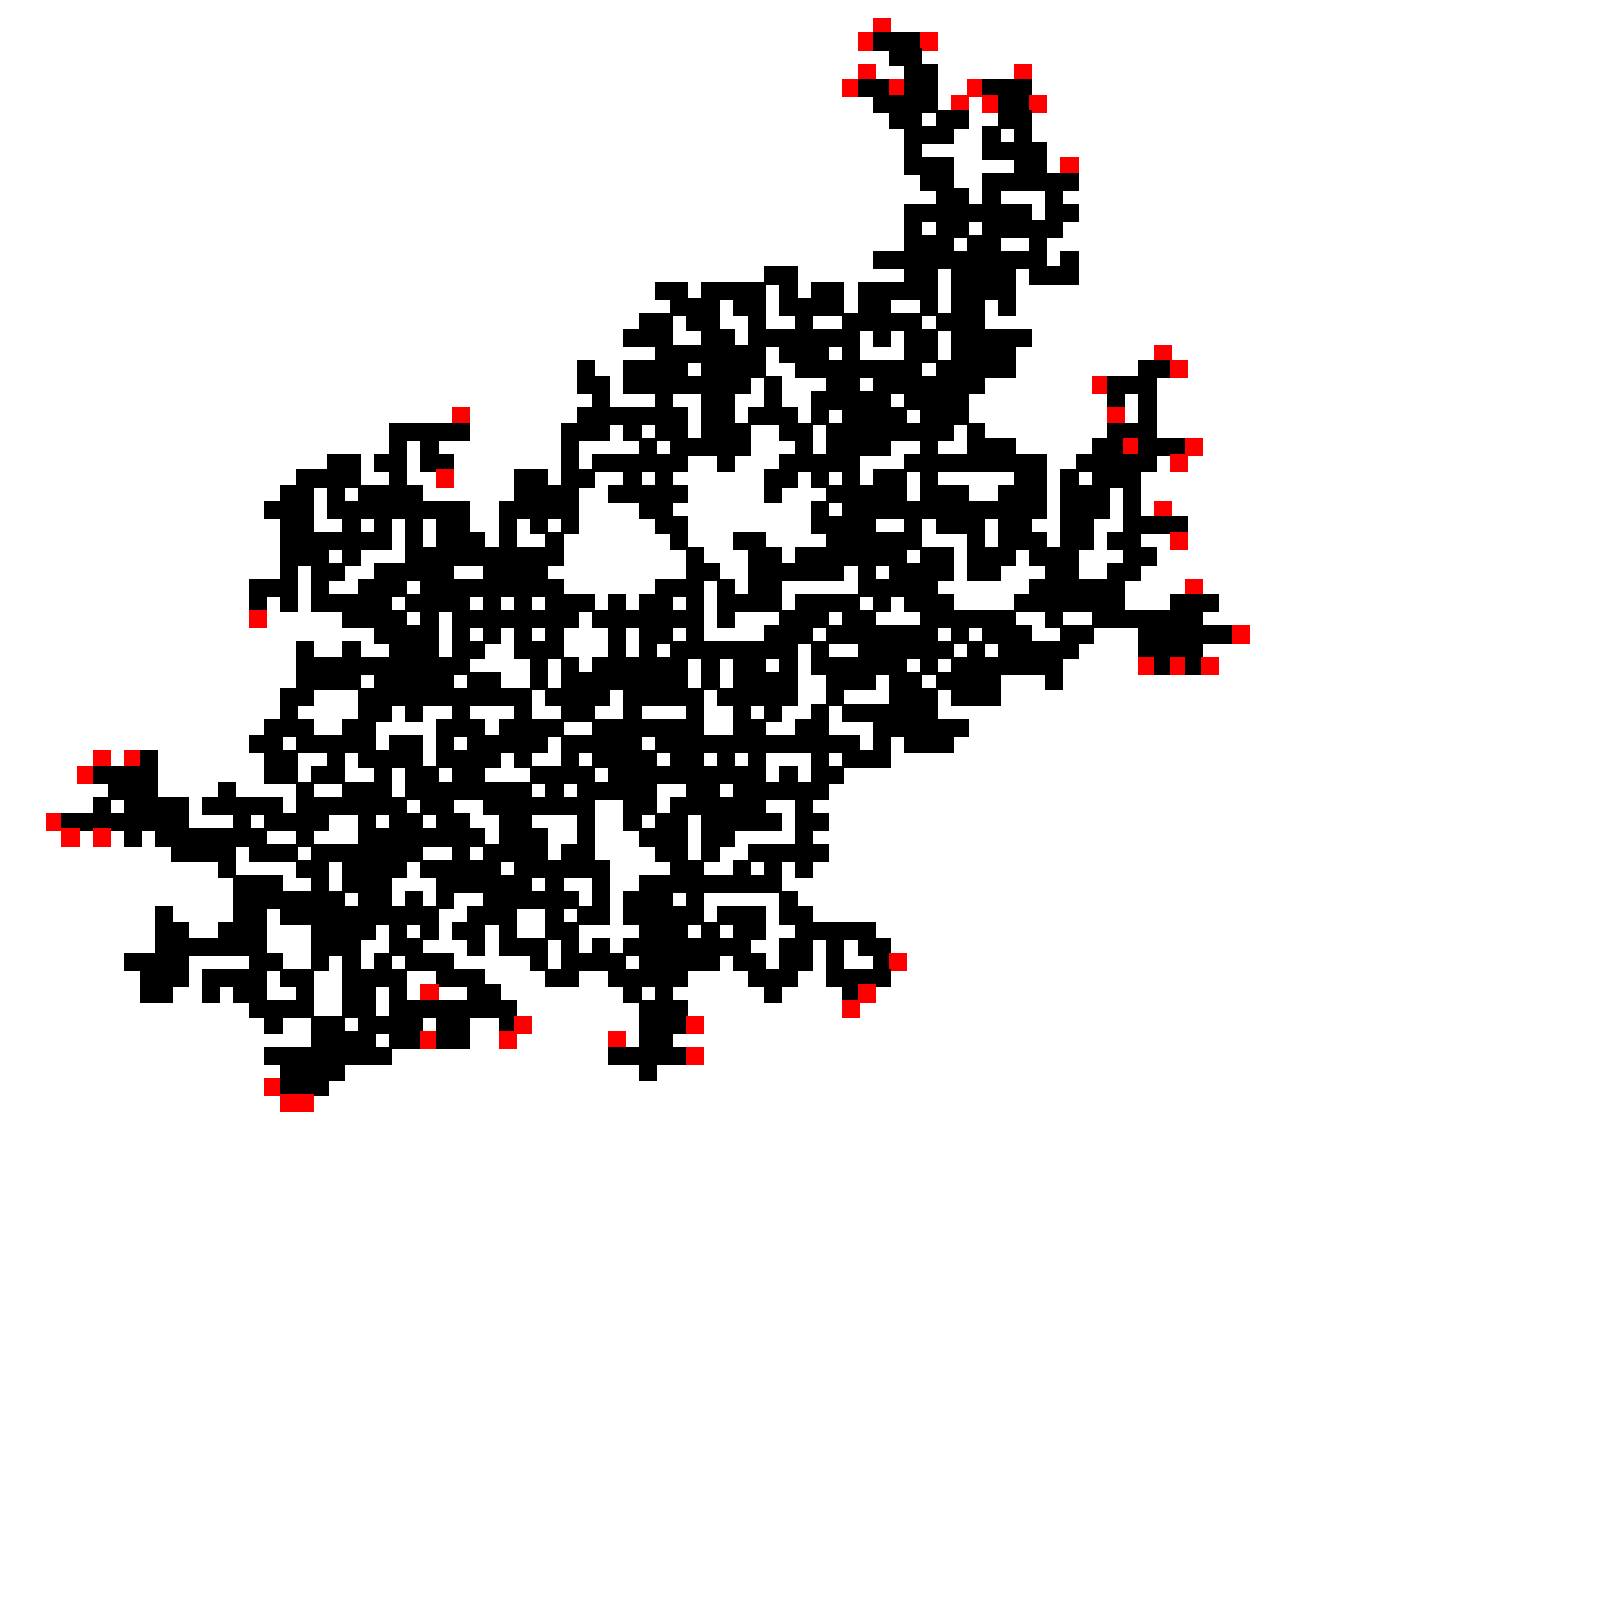
\includegraphics[width=0.3\textwidth]{bilder/eden-0.400.ps}}
  \subfigure[$p =
  0.45$]{\includegraphics[width=0.3\textwidth]{bilder/eden-0.450.ps}}
  \subfigure[$p =
  0.50$]{\includegraphics[width=0.3\textwidth]{bilder/eden-0.500.ps}}
  \caption{Eden-Simulationen mit verschiedenen Wahrscheinlichkeiten}
  \label{fig:eden}
\end{figure}



\subsection{Diffusionsbegrenzet Anlagerung (DLA)}
\label{sec:diffusionsbegrenzet_anlagerung_dla}

Hier l"asst man Teilchen im Unendlichen starten und einen Random Walk
ausf"uhren. Sobald das bewegte Teilchen an einem in der Gittermitte
sitzenden Keim ankommt, bleibt es dort sitzen und ein neuer
Random-Walk wird initialisiert.

Da Unendlich f"ur praktische Anwendungen zu weit ist, verwendet man
ca. den f"unffachen Radius der bisher erhaltenen Struktur und um
weiter Zeit zu sparen verwirft man einen Random Walk, falls dieser
sich nicht auf die Gittermitte -- wo man den ersten Keim platziert hat
-- zubewegt.

Um die so entstehenden Gebilde zu characterisieren, verwendet man den
\emph{Gyrationsradius}
\begin{equation*}
  R_g = \sqrt{ \mittel{ ( r - \mittel r )^2 } }
\end{equation*}
und die Masse $M$ (Anzahl der angelagerten Teilchen) und untersucht
nun den Zusammenhang
\begin{equation*}
  M \propto R_g^{d_f} \;,
\end{equation*}
wobei $d_f$ f"ur die \emph{Fraktale Dimension} steht. Wenn $d_f <
d_\text{Raum}$ ist, so spricht man bei dem entstandenen Gebilde von
eienm \emph{Fraktal}; da bei der DLA gew"ohnlich $d_f \approx 1.66$
haben wir hier Fraktale vorliegen.



















\backmatter



%%% Index %%%


% \newcommand{\orgtheindex}{}
% \let\orgtheindex\theindex
% \let\orgendtheindex\endtheindex
% \def\theindex{%
% \def\twocolumn{\begin{multicols}{3}}%
% \def\onecolumn{}%
% \cleardoublepage
% \orgtheindex
% }
% \def\endtheindex{%
% \end{multicols}%
% \orgendtheindex
% \cleardoublepage
% }
% 
% 
% 
% 
% \printindex












\end{document}

%%% Local Variables: 
%%% mode: latex
%%% TeX-master: t
%%% End: 
